% manuscript produces a one-column, double-spaced document:
%\documentclass[12pt,preprint]{aastex}
\documentclass[preprint]{aastex61}
%\documentclass[iop]{emulateapj}

% preprint2 produces a double-column, single-spaced document:
%\documentclass[preprint2]{aastex}

%Packages
%\usepackage[colorlinks=true,linkcolor=blue,citecolor=blue]{hyperref}

\usepackage{natbib}
\usepackage[caption=false]{subfig}
\usepackage{amsmath,amssymb}
\newcommand{\vdag}{(v)^\dagger}
\newcommand{\degree}{$^\circ$}
\newcommand{\vtan}{$V_{tan}$}
\newcommand{\kms}{km~s$^{-1}$}
\newcommand{\msun}{M$_{\sun}$}
\newcommand{\rjup}{R$_{Jup}$}
\newcommand{\ldl}{$\lambda/{\Delta}{\lambda}$}
\newcommand{\lsun}{L$_{\sun}$}
\newcommand{\lbol}{$\log_{10}{L_{bol}/L_{\sun}}$}
\newcommand{\teff}{T$_{eff}$}
\newcommand{\logg}{$\log{g}$}
\newcommand{\fsed}{$f_{sed}$}
\newcommand{\kzz}{$K_{zz}$}
\newcommand{\meth}{CH$_4$}
\newcommand{\wat}{H$_2$O}
\newcommand{\sha}{KIC 1255 b}
\newcommand{\shStar}{KIC 1255}

%\submitjournal{RNAAS}


\shorttitle{KIC 12557548 b back to normal}
\shortauthors{Schlawin et al.}


\begin{document}


\title{Back to ``Normal'' for the Disintegrating Planet Candidate KIC 12557548 b}

%% Use \author, \affil, and the \and command to format
%% author and affiliation information.
%% Note that \email has replaced the old \authoremail command
%% from AASTeX v4.0. You can use \email to mark an email address
%% anywhere in the paper, not just in the front matter.
%% As in the title, use \\ to force line breaks.

\correspondingauthor{E. Schlawin}
\email{eas342@email.arizona.edu}

\author{E. Schlawin}
\affiliation{Steward Observatory, Tucson AZ 85721}

%\author{Kento Masuda?}
%\affiliation{Department of Astrophysical Sciences, Princeton University, Princeton, NJ 08544, USA}

\author{Teruyuki Hirano}
\affiliation{Department of Earth and Planetary Sciences, Tokyo Institute of Technology, Tokyo 152-8550, Japan}

\author{Hajima Kawahara}
\affiliation{Department of Earth and Planetary Science, The University of Tokyo, Tokyo 113-0033, Japan}

\author{Johanna Teske?}
\affiliation{Department of Terrestrial Magnetism, Carnegie Institution for Science, 5241 Broad Branch Road, NW, Washington, DC 20015}

\author{Betsy Green?}
\affiliation{Steward Observatory, Tucson AZ 85721}

\author{Jonathan Fraine?}
\affiliation{Space Telescope Science Institute, 3700 San Martin Drive, Baltimore, MD 21218, USA}

\author{Rafia Bushra?}
\affiliation{Steward Observatory, Tucson AZ 85721}

\begin{abstract}
KIC 12557548 b is one of several disintegrating planet candidates which lose mass in the form of dust particles escaping their surface.
Photometric monitoring of KIC 12557548 b originally showed evidence for a slowdown of disintegration activity in 2013 and 2014.
Here, we report 2016 measurements that are consistent with photometry from the Kepler spacecraft in 2009-2013.
We also evaluate high resolution archival spectra from the Subaru HDS spectrograph and find spectra consistent with a main-sequence T=4500 $\pm$110 K star.
\end{abstract}


%\keywords{stars: atmospheres -- stars: individual (\objectname{KIC 12557548}) -- stars: variables: general}

%\section{Abstract}


\section{Introduction}
\citet{rappaport} first reported the discovery of a highly unusual stellar system in the Kepler field.
KIC 12557548's (hereafter \shStar's) light curve exhibits periodic flux dips with a period of 0.653 days.
Surprisingly, the flux dips are neither symmetric in shape nor constant in amplitude, varying from $\sim$ 0\% to $\sim$ 1.2\%.
The amplitudes of the flux dips are highly stochastic and unpredictable from one event to the next 0.653 days later.
This indicates the creation and clearing of material that can cover up to 1\% of the star in $\lesssim$ 1 day timescales.
These unusual light curve behaviors are best explained as dust extinction from material that is escaping a rocky planet (KIC 12557548 b, hereafter \sha) in a short period orbit.
The KIC 12557548 system (hereafter \shStar) has the exciting possibility of being an opportunity to study a planet that has been peeled away layer by layer to reveal an interior core.

The discovery of K2-22b \citep{sanchis-ojedak2-22}, WD 1145+017 \citep{vanderburg2015wdDisintegrating}, KOI 2700 \citep{rappaport2014KOI2700} showed that other systems have similar light curves and that other disintegrating planet systems may be useful laboratories for understanding planet evolution and composition.
Multi-wavelength light curve measurements show that the dust particles can have wavelength-dependent transmission, as predicted from sub-micron dust particles \citep{bochinski2015evolving,sanchis-ojedak2-22}.

Furthermore, there are perplexing systems that also display stochastic transit behavior but for which there are still no agreed-upon explanations: KIC 8462852 (ie. Boyajian's star) \citep{boyajian846}, RIK-210 \citep{david2017rik210} and PTFO 8-8695 \citep{vanEyken2012ptfTTauri}.
KIC 8462852 may be a family of comets from one or more parent bodies that recently were broken apart.
RIK-210 and PTFO 8-8695 are both in young systems ($\lesssim$ 10 and $\lesssim$3 Myr respectively) so they may be proto-planet candidates or structures within a protoplanetary disk.
RIK-210 could be accreting material that causes variable extinction while PTFO 8-8695's orbit may be precessing and causing variations in transit depth depending on its longitude.

The underlying planet candidate \sha\ has not been detected directly, but several observational constraints have placed upper limits on its size and mass.
High precision radial velocity measurements of the host star with Keck/HIRES put an upper limit on the reflex motion due to the planet and constrains the mass to be $\lesssim 1.2 M_{\mathrm Jup}$ \citep{croll2014}.
\citet{masuda2018rvKIC1255} find that the upper limit on the radial velocity semi-amplitude is 86 m/s corresponding to a planet mass $\lesssim 0.28 M_{\mathrm Jup}$ using the Subaru High Dispersion Spectrometer (HDS).
There is no detection of secondary eclipses of \sha\ with a 3$\sigma$ upper limit of $5 \times 10^{-5}$ in the Kepler bandpass, which means that for an albedo of 0.5, the radius of the planet must be smaller than 4600 km \citep{vanWerkhoven2014}.
A radiative-hydrodynamic wind model predicts that the mass loss rate will be a strong function of planet mass and for the present-day mass loss rate of $\sim$ M$_\oplus/Gyr$, the modeled mass is 0.014 $M_\oplus$.

One possible explanation of for the planet disintegration is that it is tied to stellar activity.
\citet{kawahara2013starspots} found an anti-correlation between stellar flux and the depth of transit events, which suggested that the alignment of the planet's position (true anomaly) causes disintegration.
The alignment of spots and disintegration activity could be due to XUV photoevaporation or magnetic reconnection events.
The anti-correlation between stellar flux and transit depth was confirmed by \citet{croll2015starspots} though they find that occultations of star spots can also modulate the transit depth at the 22.9 day rotation period of the star.

The Kepler spacecraft performed near-continuous long cadence photometry for KIC 12557548 during its entire main mission lifetime from 2009 to 2013.
During this time, the transit depths averaged around $\sim$0.6\% but varied stochastically from just one 15.7 hour orbit to the next.
\citet{vanWerkhoven2014} analyzed 15 of the total 17 quarters of data and calculated every transit depth during this period.
There were two intervals near obits 50 and 1950 that showed shallower (0.1\%) than average transit depths for roughly one month in duration.

The Kepler data was used to put constraints on the particle size distribution and composition of the dust particles.
\citet{budaj12} and \citet{brogi2012} modeled the light curve, which includes a slight increase in flux prior before the transit begins.
This pre-ingress flux increase is caused by forward scattering dust particles and the scattering function is sensitive to particle size modulo composition.
\citet{budaj12} and \citet{brogi2012} find particle sizes $\sim$0.1 to $\sim$1.0$\mu$m in size based on this method.
Subsequently, \citet{croll2014} obtained a $K'$-band light curve simultaneously with the Kepler spacecraft to put a constraint on the dust extinction as a function of wavelength.
\citet{croll2014} find a particle size distribution of $\gtrsim 0.5\mu$m.

\citet{schlawin2016kic1255} observed 8 total transits of the system for 4 nights in 2013 and 4 nights in 2014 for the $r'$ band using the MORIS imager \citep{Gulbis2011} on SpeX/IRTF \citep{rayner03}.
\citet{schlawin2016kic1255} found that the optical transit depths were all weaker than $0.43\%$ and that the probably of this randomly occurring based on random behavior from Kepler statistics was around 0.2\%.
This was evidence that the observations occurred during weaker periods (as found in \citet{vanWerkhoven2014}'s 15 Kepler quarter analysis) or that the disintegration activity was falling off with time.
We performed follow-up $R$ band photometry of the \shStar\ system to explore these two hypotheses and see if the the disintegration has returned to the levels found in the Kepler mission.

The high resolution spectrum of \shStar\ \citep{kawahara2013starspots} showed a different temperature and gravity than photometric methods \cite[e.g.][]{brown2011kic}.
\citet{vanlieshout2016kic1255} suggest that one exciting possibility is that gases from the disintegrating planet contaminate the high resolution spectrum.
This would enable compositional and kinematic studies of the disintegrating planet.
Here, we examine archival Subaru High Dispersion Spectrograph (HDS) spectra of the star to assess the stellar parameters and explore the possibility that sublimated gases appear in the high resolution spectrum.

\begin{deluxetable}{lrr}
\tablecaption{List of photometric observations}\label{tab:photSummary}
\tablewidth{0pt}
\tablehead{
\colhead{Date} &
\colhead{Weather} &
\colhead{Amplitude} \\
\colhead{UT} & & \\
 }
\startdata
2016 Jun 10 & Clouds	& \nodata \\
2016 Jun 12 & Clear 		& 0.94 $\pm$ 0.16 \\
2016 Jun 14 & Clear 		&0.70 $\pm$ 0.18\\
2016 Jul 12 & Clear 		& 0.78 $\pm$ 0.14 \\
2016 Jul 14 & Mostly clear	& 1.33 $\pm$ 0.14 \\
2016 Jul 16 & Clear 		& 2.14 $\pm$ 0.19 \\
\enddata
\tablenotetext{}{Summary of the attempted photometric observations of \shStar\ with the 61-inch Kuiper observatory.}
\end{deluxetable}

\section{Observations}
We attempted to observe 6 transit events of \sha\ with the Mont4k imager on the 61-inch Kuiper observatory located on Mt Bigelow, Arizona on UT using the f/13.5 Cassegrain focus.
On all nights we used 90 second exposures using a Harris-R filter to best approximate the $r'$ filter used in \citet{schlawin2016kic1255}.
5 of the 6 nights were clear with the exception of a few passing clouds on UT 2016 Jul 14.
Cloudy skies on UT 2016 Jun 10 that prevented high precision time series.
Table \ref{tab:photSummary} shows a summary of our observations and the UT dates.
The data was taken in a 3x3 binning mode resulting in an effective 0.43"/pixel plate scale.

\subsection{Photometric Pipeline}

For the photometric reduction, we used the Python \texttt{ccdproc} package \citep{craig2015ccdproc} to generate master flat field and bias files.
They were combined with an average with a low threshold of 2$\sigma$ and a high threshold of 5$\sigma$.

We used the Python \texttt{photutils v0.3} \citep{bradley2016photutilsv0p3} package to centroid and extract fluxes of the \shStar\ and the reference stars.
We used a photometric aperture of 9 pixels (3.9") and a background annulus from 9 to 12 pixels (3.9" to 5.2") on all stars and nights.
12 stable reference stars with similar R band brightnesses were used to construct a reference time series to correct for variable telluric and instrument throughput.
The reference stars are identified Figure \ref{fig:refStars} across the 9.8\arcmin $\times$ 9.8 \arcmin\ Mont4K field of view.
These 12 reference stars' time series were combined with a weighted average and this combined time series was divided into the target, \shStar.

\begin{figure}
\begin{centering}
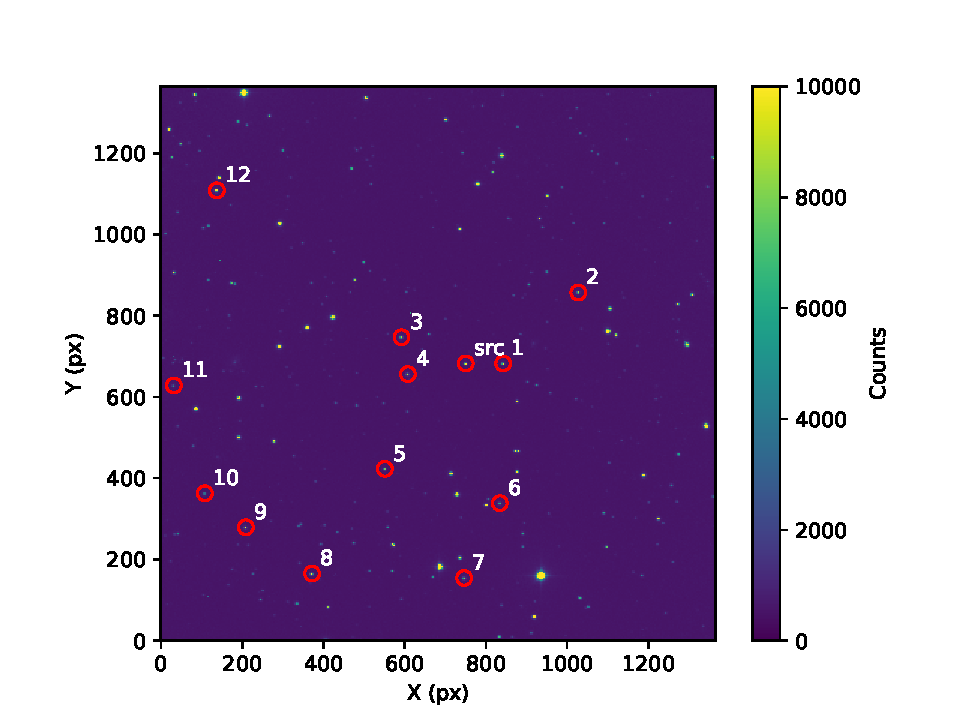
\includegraphics[width=0.49\textwidth]{images/ut2016_07_14_clouds/figure_index_152.pdf}
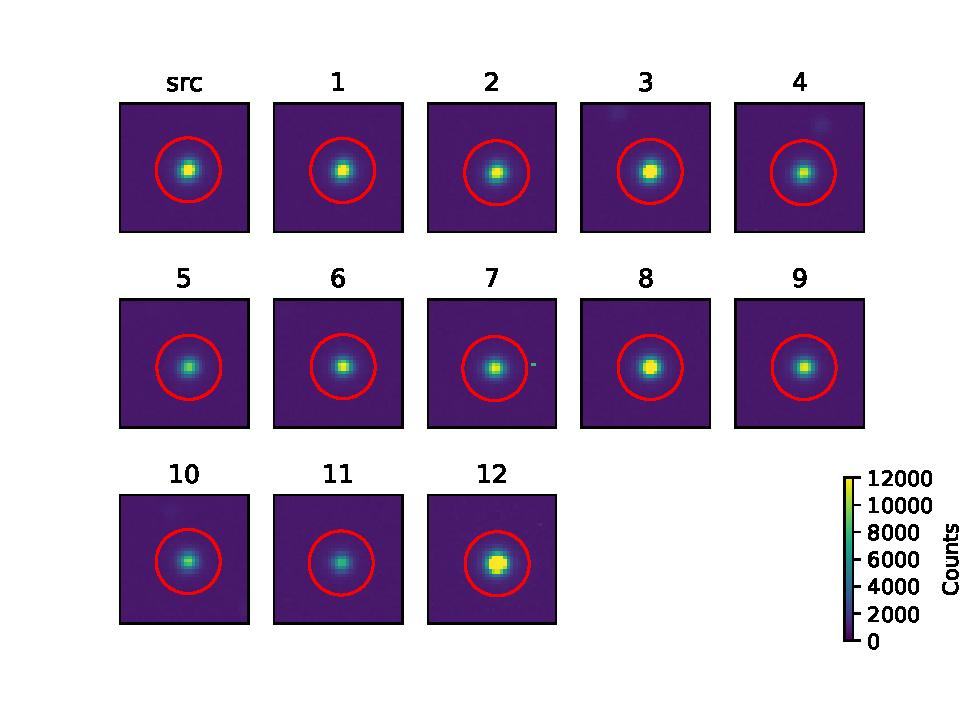
\includegraphics[width=0.49\textwidth]{images/stamps_kic1255_UT2016_07_14.pdf}
\caption{{\it Left:} \shStar\ (src) and reference stars (numbered) used on UT 2016-07-14 are shown over the full 9.8\arcmin $\times$ 9.8\arcmin\ Field of View of Mont4K.
{\it Right:} Postage stamp zoom-ins for the source and reference stars show the point spread functions for each star.
The reference stars were chosen to have similar count levels as \shStar.
}\label{fig:refStars}
\end{centering}
\end{figure}

All light curves for \shStar\ and the 12 reference stars are shown in Figure \ref{fig:allNightallStar}.
These are the same reference stars shown in Figure \ref{fig:refStars}.
The two nights 2016 Jun 12 and 2016 Jun 14 show greater overall stability than the 3 nights in July, 2016.
We suspect that the higher moisture levels and occasional cloud passages (such as the ones that caused huge drops in flux on UT 2016 Jul 14) affected the later observations.

\begin{figure*}
\begin{centering}
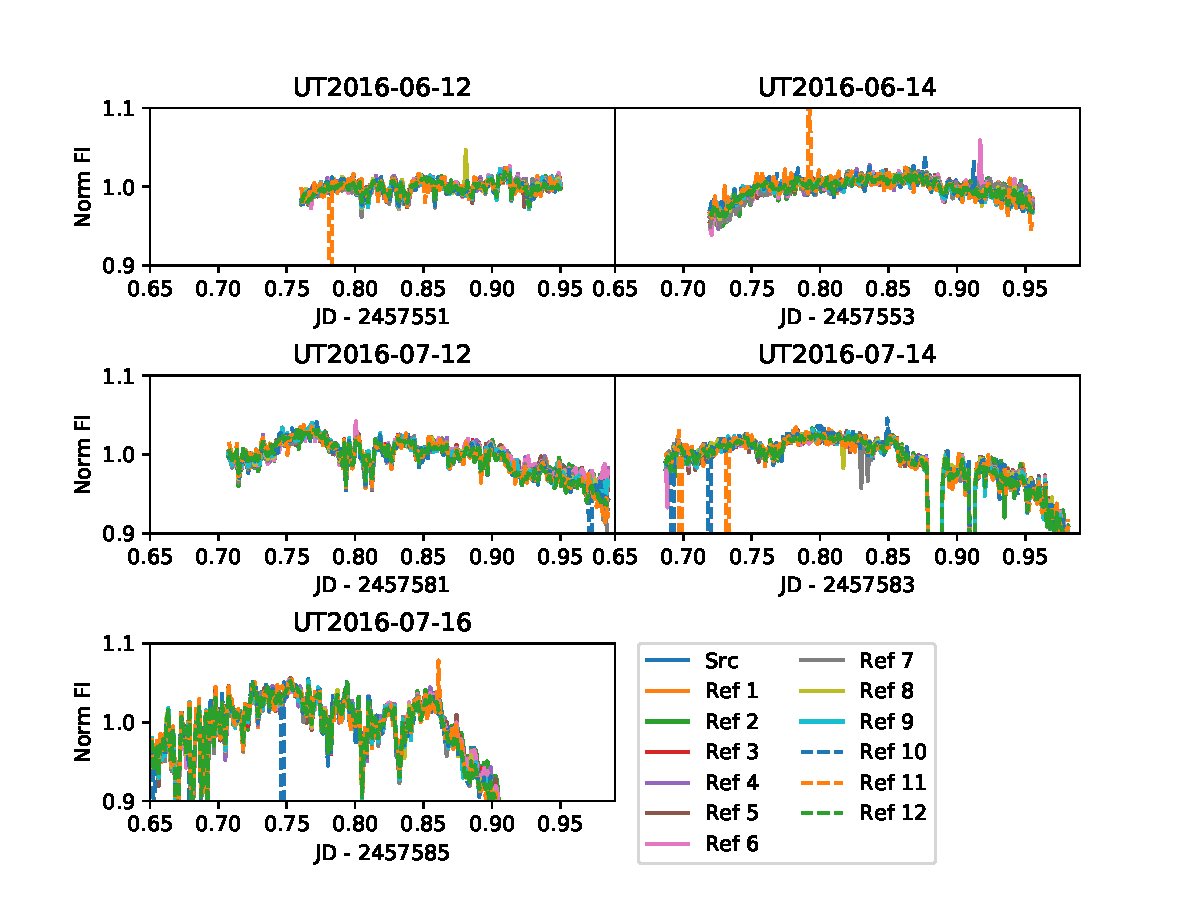
\includegraphics[width=0.9\textwidth]{images/all_kic1255_phot/all_kic1255_allstar.pdf}
\caption{Time series photometry for all stars and all nights nights.
The nights in July appear more strongly affected by cloud/and or seeing variations, whereas the two nights in June are stable to within a few percent.
All source radius, background start and background annulus end parameters were 9, 9 and 12 pixels respectively.}\label{fig:allNightallStar}
\end{centering}
\end{figure*}

Figure \ref{fig:allNightrefCorrect} shows the reference-corrected time series for \shStar\ for all nights.
We use the planet transit ephemeris from \citet{croll2015starspots} where the Kepler flux minimum is the ``transit center'':
\begin{equation}
T = T_0 + n P
\end{equation}
where $T_0 = 2 454 968.982 0 \pm 0.000 7$ BJD$_{TDB}$ and $P = 0.653 553 4 \pm 0.000 000 2$ days.
The expected transit epochs from the ephemeris in \citep{vanWerkhoven2014} are shown for reference as vertical red bars.
Typical uncertainties for the Kepler ephemeris are $\sim$ 1 minute at these dates due to the large number of transits measured by the Kepler observatory over nearly 4 years.
The ``transit duration'' from Kepler light curves is around 0.05 days, which is consistent with these transit durations.

We also overlay the average Kepler short cadence light curves on the measured light curves.
To ease the comparison of the average Kepler light curve and measured data, we bin the 61-inch Mont4K data into 20 minute long bins.
Obvious cosmic ray outliers were discarded by removing points with fluxes below 0.98 and above 1.02 times the median flux.
The error bars for the binned data are calculated from the standard error in the mean for each bin.
When comparing the average Kepler Short Cadence light curve and the measured light curves that the measured light curves represent typical KIC 12557548 b transits.
Only 2016-06-14 appears to have a non-detection.

\begin{figure*}
\begin{centering}
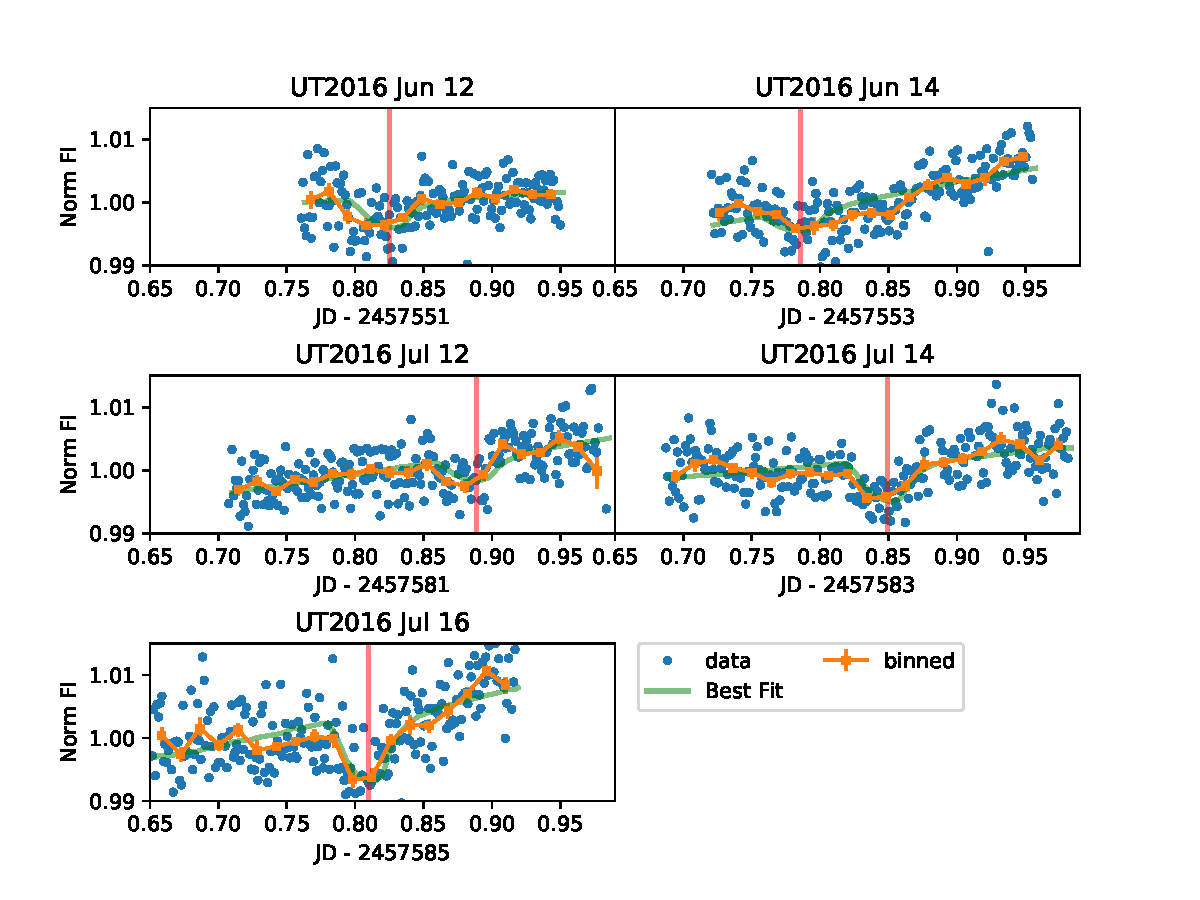
\includegraphics[width=0.9\textwidth]{images/all_kic1255_phot/all_kic1255_refcor.pdf}
\caption{Reference-corrected time series photometry \shStar\ for all nights (blue circles).
Orange squares mark 20 minute flux bins.
The expected transit epochs from the Kepler-based ephemeris \citep{vanWerkhoven2014} are shown as vertical red bars.
We also show the average Short Cadence Kepler light curves for each of the transit events for comparison with the average.
Transits are clearly visible for all five nights except for UT2016-06-14.}\label{fig:allNightrefCorrect}
\end{centering}
\end{figure*}

\clearpage

\section{Stellar Characterization}
\subsection{Previous Observations}

\begin{deluxetable*}{lcrrr}
\tablecaption{Observational estimates of the stellar parameters of \shStar, adapted from \citet{vanlieshout2016kic1255}}
\tablewidth{0pt}
\tablehead{
\colhead{Reference} &
\colhead{$ T_{eff,*} $} &
\colhead{$\log(g)$} &
\colhead{Evolutionary Status} &
\colhead{Method} \\
 & (K) & $\log$(cm s$^{-2}$) & & \\
 }
\startdata
  \citet{brown2011kic} & 4400 $\pm$ 200   & 4.6 $\pm$ 0.5    & main-sequence star & photometry \\
  \citet{rappaport}       & 4300 $\pm$ 250    &                            & main-sequence star & low-resolution spectroscopy \\
  \citet{kawahara2013starspots} & 4950 $\pm$ 70 & 3.9 $\pm$ 0.2 & sub-giant          & high-resolution spectroscopy \\
  \citet{huber2014kicprop} & 4550$^{+140}_{-131} $ & 4.622$^{+0.043}_{-0.036} $& main-sequence star & photometry \\
  \citet{morton2016falsePos} & 4677 		& 4.61		& main-sequence star	& photometry \\
  \citet{vanlieshout2016kic1255} & 		& $\gtrsim 4.4$	& main-sequence star	& transit light curve \\
  This work - Specmatch	& 4500 $\pm$110 	& 4.63 $\pm$ 0.1 & main-sequence star & high-resolution spectroscopy\\
  This work - BOSZ		& 4500	& 4.5		& main-sequence star & high-resolution spectroscopy\\
\enddata
\tablenotetext{}{While most of the photometric results show a surface gravity of a main sequence star, the high resolution analysis from \citet{kawahara2013starspots} indicates a gravity consistent with a sub-giant star.}\label{tab:stellObsParams}
\end{deluxetable*}


The host star \shStar\ has been characterized by both photometry and spectroscopy to better understand the system and parameters of the disintegrating planet and debris.
Table \ref{tab:stellObsParams} shows the summary of observations and analyses compiled in \citet{vanlieshout2016kic1255} for the stellar properties, re-produced here with additional results added from \citet{morton2016falsePos} and this work.
In the photometric analysis and low resolution spectroscopy, the spectra are consistent with a 4500 K main sequence K-type star.
High resolution spectra, however, indicated a higher temperature 4900 K lower log(g) sub-giant star \citep{kawahara2013starspots}.
\citet{vanlieshout2016kic1255} analyzed the light curve with a dust model to put constraints on the semi-major axis in terms of stellar radii, which can be combined with Kepler's third law to calculate the stellar density \citep{seager2003uniqueSolution}.
\citet{vanlieshout2016kic1255} find that the stellar density is only consistent with a main-sequence star with log(g) $\gtrsim 4.4 \log($cm s$^{-2})$.
They suggest an intriguing possibility that the high resolution spectrum of \shStar\ has contamination from dusty debris from the planet and thus appears as a sub-giant star.
If true, high resolution spectra would be valuable tool to study the composition and dynamics of the material escaping \sha.
In this section, we analyze archival high resolution spectra to put new constraints on the stellar temperature and surface gravity.

\subsection{Subaru HDS Spectra}\label{sec:SubaruDescrip}

We evaluate the stellar parameters by examining the archival spectra taken with the High Definition Spectrograph (HDS) spectrograph on the Subaru telescope \citep{noguchi2002hds}.
An observing log of the 3 nights is summarized in Table \ref{tab:specObs}.
There is one set of data taken on 2013 June 22 (UT) discussed in \citet{kawahara2013starspots}, including 2 exposures each 2700 seconds in duration.
For this 2013 observation, the instrument was configured to use an image slicer unit \#2, which has a resolving power R$\approx$80,000.
Additionally, there are two sets of observations from 2015 Aug 28 (UT) and 2015 Aug 29 (UT) that were taken to test if the planet could be on a high eccentricity grazing orbit \citep{masuda2018rvKIC1255}, with exposure durations of 2400 seconds each.
The instrument was configured with a 0.3 mm (0.6\arcsec) wide and 30 mm long (60\arcsec) slit, which has a resolving power of R $\approx$60,000.
The second set of observations happened after the reaction wheel failure on 2013 May 11\footnote{\url{https://www.nasa.gov/mission_pages/kepler/news/keplerm-20130521.html}} that ended photometry of the main Kepler field, so no simultaneous Kepler photometry was available with the high dispersion spectroscopy to assess disintegration activity preceding or following the spectra.
None of the observations was timed during a primary transit (phase = 0.0) or secondary eclipse (phase = 0.5 for a circular orbit).

\begin{deluxetable}{cccccccc}
\tablecaption{List of Spectroscopic Observations}
\tablefontsize{\scriptsize}
\tablehead{\colhead{Exposure Number} & \colhead{ExpTime} & \colhead{UT Date} & \colhead{UT Start} & \colhead{Image Slicer} & \colhead{Slit Width} & \colhead{Orbital Phase} & \colhead{Resolving Power}\\
	& (s)	& & & & (mm) & & R}
\startdata
94085 & 2700 & 2013 Jun 22 & 12:32 & 2 & 2.0 & 0.621 & 80,000 \\
94087 & 2700 & 2013 Jun 22 & 13:18 & 2 & 2.0 & 0.670 & 80,000 \\
111345 & 2400 & 2015 Aug 28 & 05:37 & N & 0.3 & 0.667 & 60,000 \\
111349 & 2303 & 2015 Aug 28 & 06:19 & N & 0.3 & 0.712 & 60,000 \\
111355 & 2400 & 2015 Aug 28 & 07:33 & N & 0.3 & 0.790 & 60,000 \\
111359 & 2400 & 2015 Aug 28 & 08:15 & N & 0.3 & 0.835 & 60,000 \\
111373 & 2400 & 2015 Aug 28 & 09:17 & N & 0.3 & 0.901 & 60,000 \\
111525 & 2400 & 2015 Aug 29 & 05:34 & N & 0.3 & 0.194 & 60,000 \\
111529 & 2400 & 2015 Aug 29 & 06:17 & N & 0.3 & 0.240 & 60,000 \\
111533 & 2400 & 2015 Aug 29 & 07:00 & N & 0.3 & 0.285 & 60,000 \\
111549 & 2400 & 2015 Aug 29 & 08:31 & N & 0.3 & 0.382 & 60,000 \\
111553 & 2400 & 2015 Aug 29 & 09:14 & N & 0.3 & 0.428 & 60,000 \\
\enddata
\tablenotetext{}{Observing log of the Subaru HDS spectroscopic observations.}\label{tab:specObs}
\end{deluxetable}


\subsection{Data Reduction}
For the 2015 data, we use the same spectra as in \citep{masuda2018rvKIC1255}.
All telluric emission features and outliers are masked in this analysis to remove these components.
Time-variable outliers like cosmic rays are removed by measuring deviations from the median spectrum for the night.
The night-sky emissions from OH and O$_2$ are removed by using the \citet{osterbrock1996lineAtlas} night sky atlas.
All OH and O$_2$ lines are removed regardless if they are visible in the spectrum of \shStar.
To combine the observations, we found the median spectrum for UT dates 2015 Aug 28 and 2015 Aug 29 to robustly combine the data.
This median spectrum is visible in Figure \ref{fig:mgTripletBOSZ}.

For the 2013 data, we follow the \texttt{iraf} reduction techniques from the instrument manual V2.0.0  \footnote{\url{https://www.subarutelescope.org/Observing/Instruments/HDS/}}.
Some modifications to the manual were made, including a more aggressive -50/+50 lower and upper window for bad pixel identification with \texttt{mkbadpx} on the red CCD.
We applied bad pixel masks and bias files to each CCD (red and blue sides) separately.

We performed wavelength calibration with a Thorium Argon reference spectrum.
The final wavelength calibration fit was performed with a chebyshev polynomial, 4th order in x direction and 4th order in y direction.
This polynomial fit has a RMS error of 0.02$\AA$.

We compare the 2013 and 2015 data to search for any variability in the absorption lines, as seen in Figure \ref{fig:spec2013vs2015}.
Absorption line variability could be caused by disintegration activity of the planet that escapes as dusty material and then sublimates into gas.
This gas absorption could provide kinematic information on escaping material provided that the sublimated gas has sufficient optical depth.
We find no statistically significant differences between the 2013 and 2015 spectra, as shown in Figure \ref{fig:spec2013vs2015}.
We then proceed with the 2015 data to constrain stellar models since it has 6.7 hours of total exposure time compared (compared to 1.5 hours in 2013).

\begin{figure*}[!hbtp]
\begin{centering}
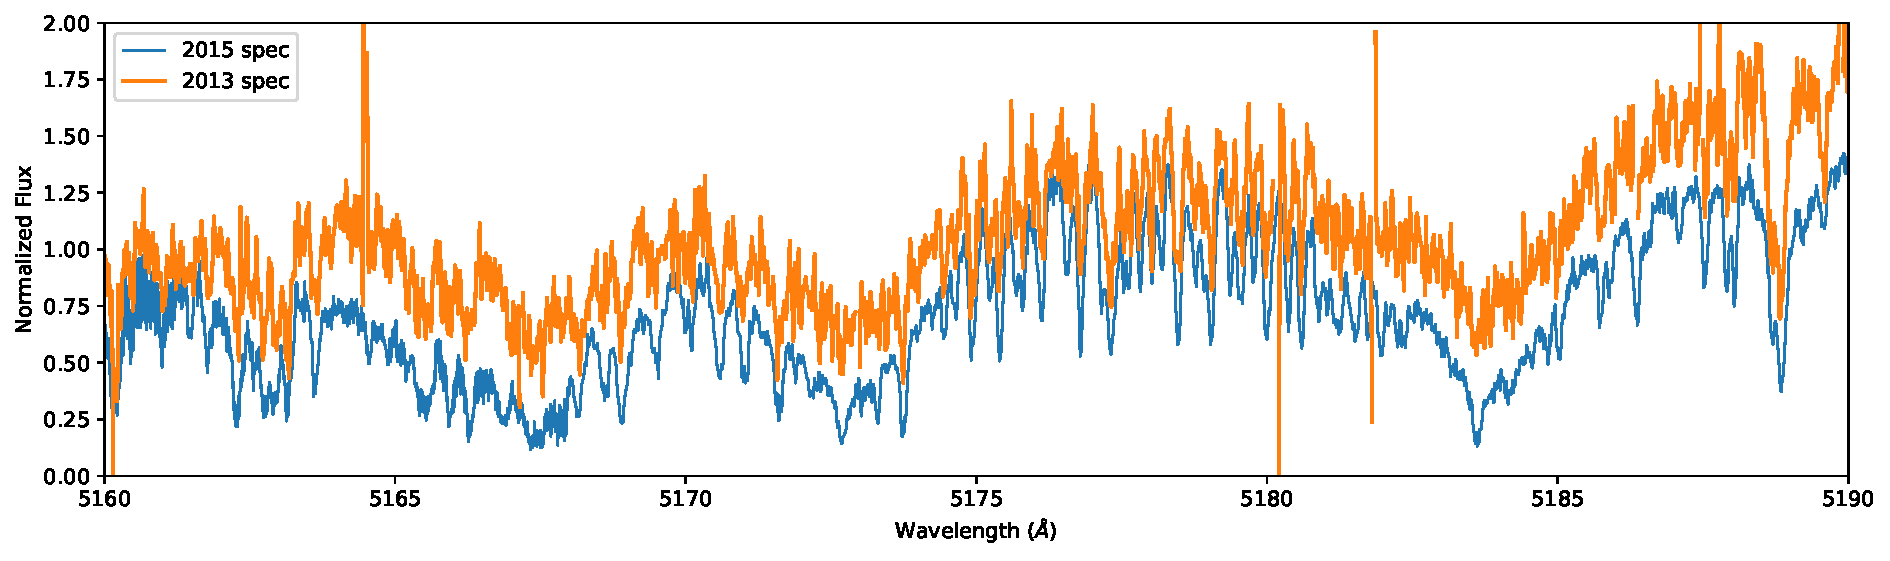
\includegraphics[width=1.0\textwidth]{images/subaru/2013_vs_2015/2013_vs_2015_spec.pdf}
\caption{Comparison between the 2013 spectrum and 2015 median spectrum of \shStar\ near the Mg I triplet. The two are consistent within the larger noise of the 2013 data.}\label{fig:spec2013vs2015}
\end{centering}
\end{figure*}

\subsection{Comparison to BOSZ}
We first evaluate stellar parameters by comparing to the high resolving power ($R=100,000$) BOSZ grids of ATLAS-APOGEE ATLAS9 models \citep{bohlin2017bosz} to the median spectrum from 2015.
Since the discrepancies in the literature are mostly differences in the surface gravity (see Table \ref{tab:stellObsParams}), we study the gravity-sensitive Mg triplet near 517 nm.
The $R=100,000$ models are convolved with a Gaussian kernel that has a standard deviation $\sigma_K = \lambda/161,000 \approx 0.03 \AA$ to best match the data.
This was a smaller we expected from combining inverse resolving powers in quadrature, which would imply that an $R=75,000 $ kernel convolved with an $R=100,000$ spectrum would result in a $R=60,000$ spectrum.
We start by comparing the measured spectrum with two BOSZ models in Figure \ref{fig:mgTripletBOSZ}.
Here, the two BOSZ models are broadly representative of the two types of results in Table \ref{tab:stellObsParams} (log(g)=4.5 and log(g)=4.0).
The higher gravity log(g)=4.5 model appears to match the data better in terms of line ratios but does not explain all of the line depths in the spectrum.

\begin{figure}[!hbtp]
\begin{centering}
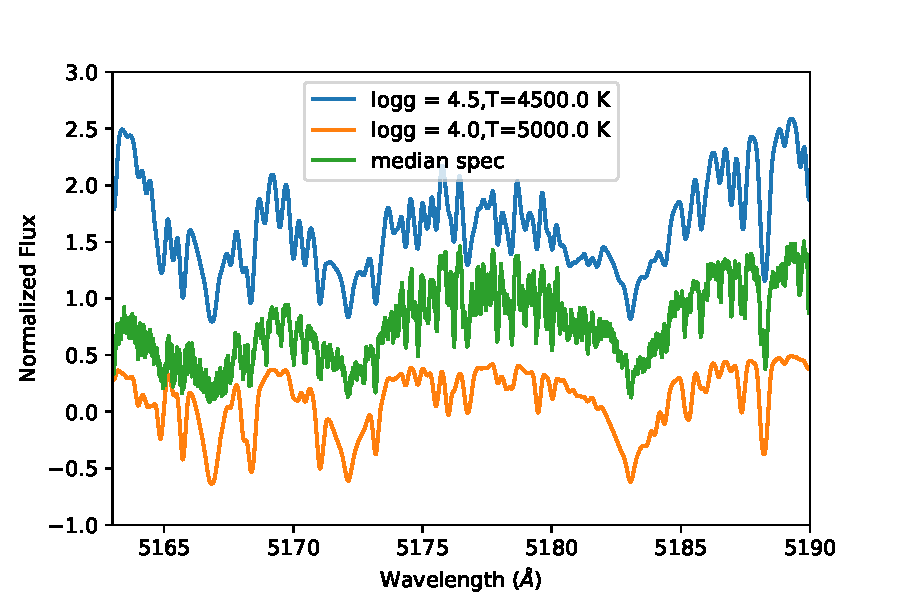
\includegraphics[width=0.7\textwidth]{images/subaru/bosz_mg_triplet_median_spec_w_5000.pdf}
\caption{Median spectrum of \shStar\ \citep{masuda2018rvKIC1255} near the Mg triplet compared to 4500 K BOSZ models with two different log(g)s.}\label{fig:mgTripletBOSZ}
\end{centering}
\end{figure}

We explore the 5 parameters in the BOSZ models: T$_{eff}$, log(g), [M/H], [$\alpha$/M] and [C/M] to constrain these parameters in \shStar.
The sensitivity to each parameter for the BOSZ models are shown in Figure \ref{fig:boszModelParamsMedianSpec}.
For each parameter, we change the models by about 2 steps in the BOSZ grid.
For a quantitative measure of the goodness-of-fit, we calculate a $\chi^2$ over the Mg triplet lines from 5160 to 5190 $\AA$.
The errors are estimated from the standard deviation of the spectra over the night.

%A temperature near 4500 K, log(g) = 4.0-4.5, high metallicity ([M/H] $\approx$ 0.5), low $\alpha$ enrichment ($\alpha \approx -0.25$ and solar Carbon to metals ([C/M] $\approx$ 0) are favored by the models.

\begin{figure*}[!hbtp]
\begin{centering}
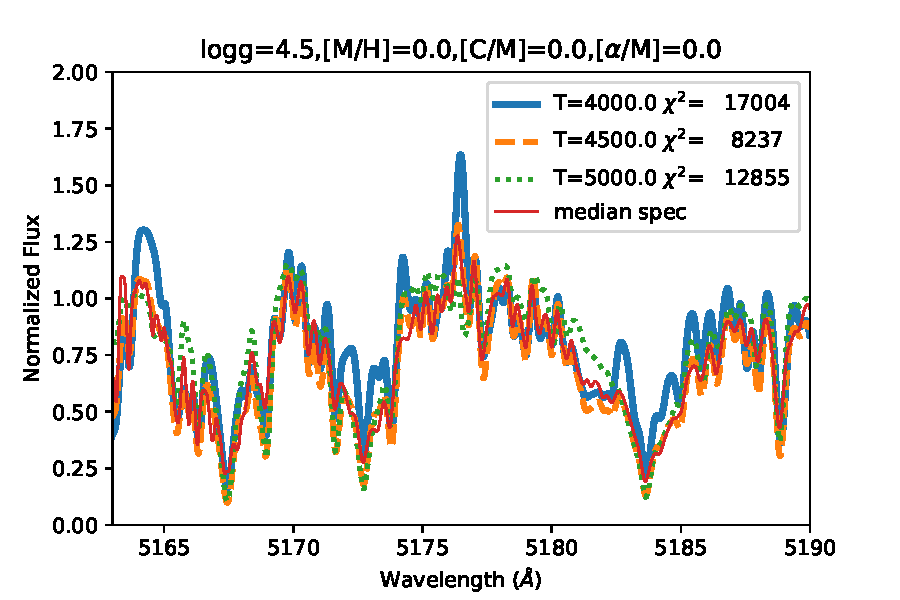
\includegraphics[width=0.45\textwidth]{images/bosz_model_exploration/T_EFF_exploration.pdf}
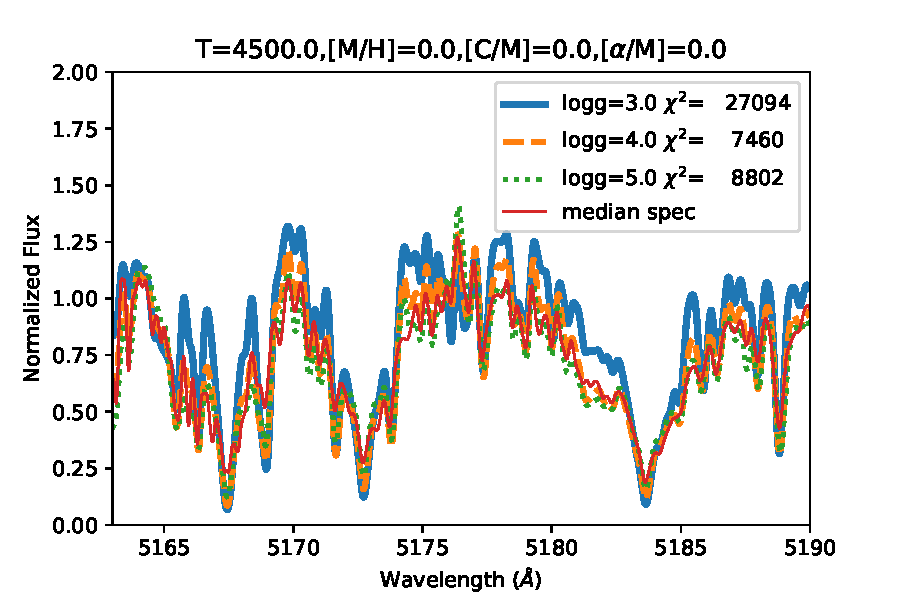
\includegraphics[width=0.45\textwidth]{images/bosz_model_exploration/LOGG_exploration}
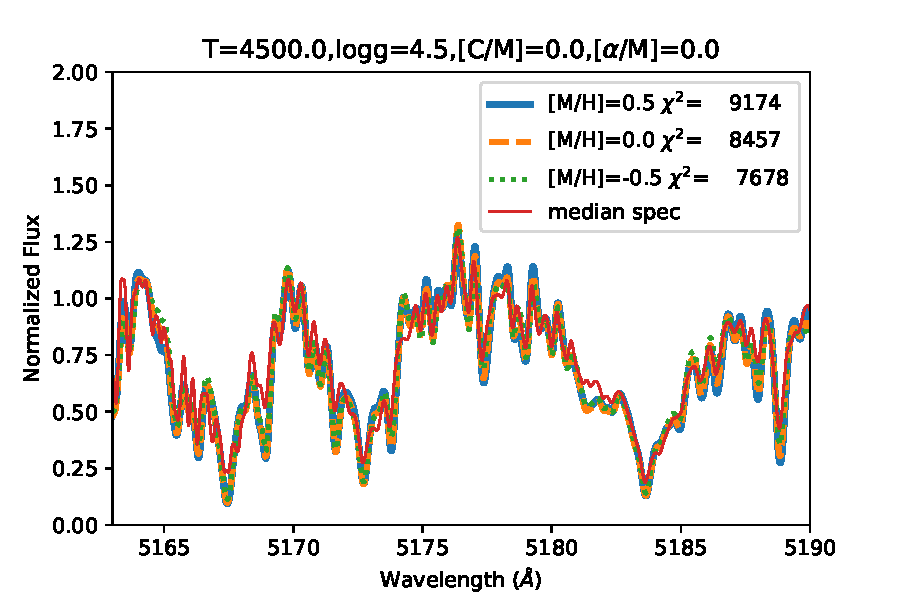
\includegraphics[width=0.45\textwidth]{images/bosz_model_exploration/MH_exploration.pdf}
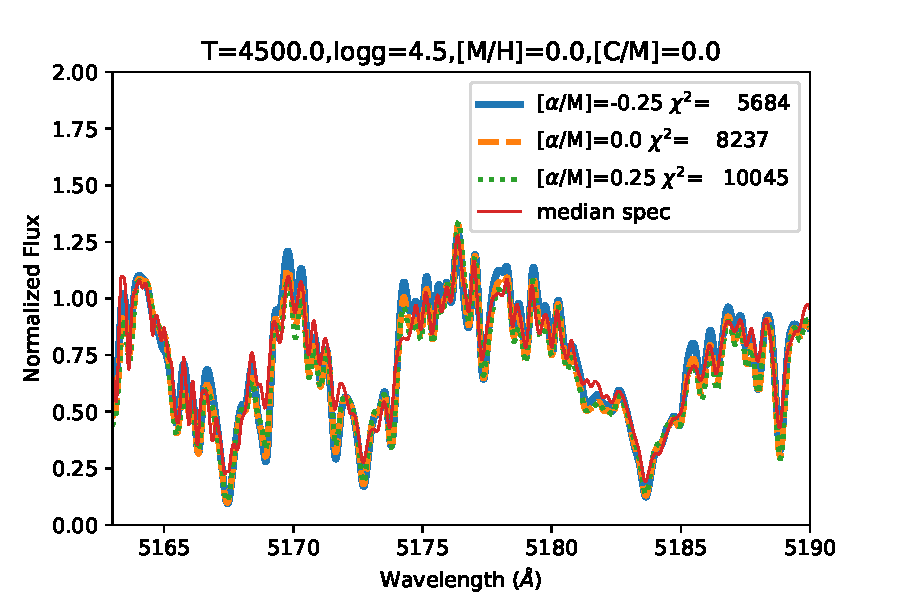
\includegraphics[width=0.45\textwidth]{images/bosz_model_exploration/ALPHA_exploration.pdf}
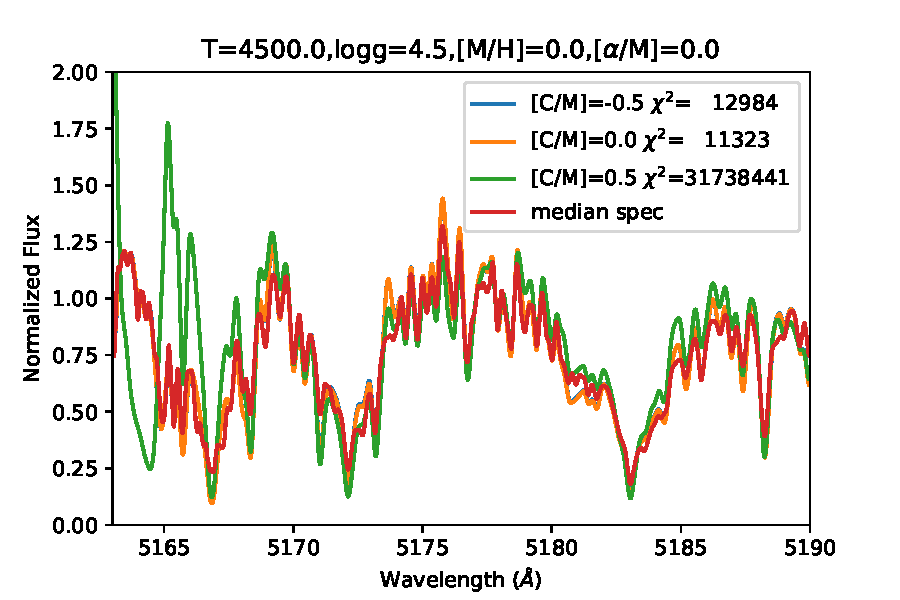
\includegraphics[width=0.45\textwidth]{images/bosz_model_exploration/CM_exploration.pdf}
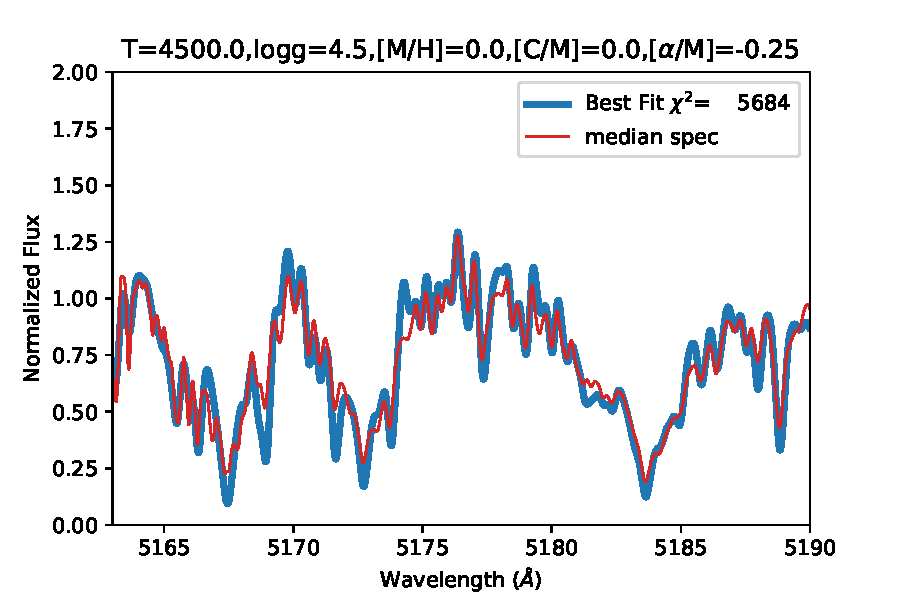
\includegraphics[width=0.45\textwidth]{images/bosz_model_exploration/FINAL_exploration.pdf}
\caption{The BOSZ models are explored over the parameter space to search for a best fit as well as visualize how much each parameter affects the spectrum.
The bottom right plot shows the best-fit BOSZ model, but it still under-predicts and over-predicts some line strengths.}\label{fig:boszModelParamsMedianSpec}
\end{centering}
\end{figure*}

After initial constraints on the models from the sensitivity to parameters search, we downloaded a grid of BOSZ models with temperatures ranging from 4250 K to 4750 K, Log(g) from 4.0 to 4.5, [M/H] from 0.0 to 0.5, [C/M]=0.0 and [$\alpha$/M] = -0.25 to 0.0.
We found the model with the  $\chi^2$ statistic over the Mg triple lines from 5160 to 51690 $\AA$
As discussed above, we use an approximate $\chi^2$ statistic over the wavelength range covering the Mg triplet (5160 $\AA$ to 5190 $\AA$).
The minimum $\chi^2$ model for this entire grid is the same as shown in Figure \ref{fig:boszModelParamsMedianSpec} on the Bottom Right: T=4500 K, Log(g)=4.5, M/H=0.0, C/M=0.0, $\alpha=-0.25$.
This is similar to the log(g)$\approx$4.6, T=4500 stellar parameters derived from photometry and low resolution spectroscopy listed in Table \ref{tab:stellObsParams}.

\subsection{SpecMatch-Emp}\label{sec:SpecMatch-Emp}

We also use the open-source \texttt{SpecMatch-Emp} tool \citep{yee2017specMatch} to estimate the stellar parameters using the Subaru spectrum.
\texttt{SpecMatch-Emp} uses a library of Keck HIRES spectra to match the spectrum and derive stellar parameters.
%The median spectrum from 2015 has a resolution of $R=60,000$, which is close to the \texttt{SpecMatch-Emp} grid of $R=55,000$, so we do not convolve the input data for \texttt{SpecMatch-Emp}.
We cut the spectrum to a region from 5140~$\AA$ to 5190~$\AA$ to focus on the gravity-sensitive Mg triplet.

Figure \ref{fig:SpecMatch-Emp} shows the chi-squared differences between the median Subaru spectrum and the models.
The effective temperature and radius parameters show clear global $\chi^2$ minima for the HIRES spectral libraries.
However, the metallicity is less well constrained.
The resulting best-fit parameters from \texttt{SpecMatch-Emp} are T$_{eff}$=4500 K $\pm$ 110 K, [Fe/H]=-0.1$\pm$0.1, log(g)=4.5$\pm$0.1, R=0.7 $\pm$ 0.1 R$_\odot$ and Mass=0.7 $\pm 0.1 $M$_\odot$.
The output \texttt{SpecMatch-Emp} age constraint of 9.6 $\pm$ 0.2 Gyr is likely an underestimated error in the age.
Figure \ref{fig:SpecMatch-EmpComb} shows the linear combination of spectra that best-fit \shStar\ from \texttt{SpecMatch-Emp}.

\begin{figure*}[!hbtp]
\begin{centering}
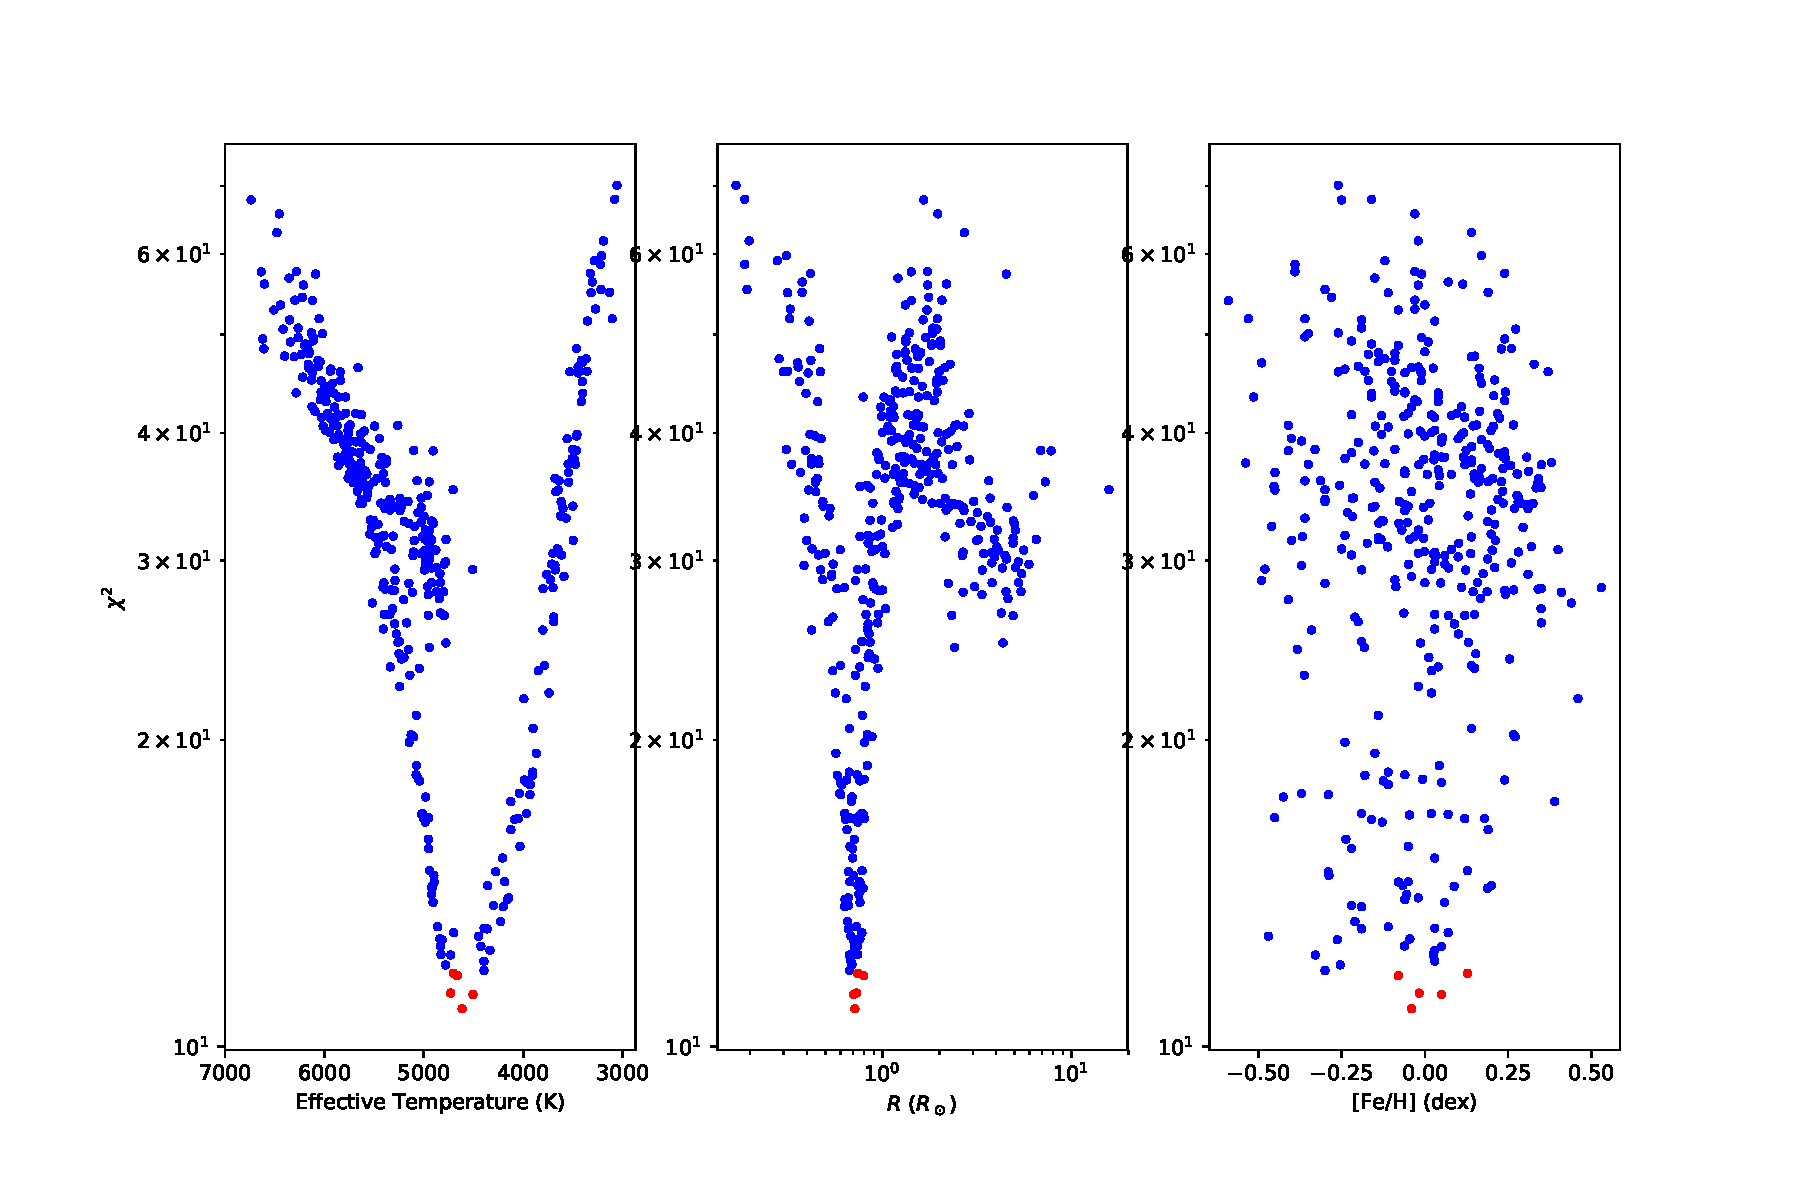
\includegraphics[width=0.8\textwidth]{images/subaru/spec_chi_min.pdf}
\caption{$\chi^2$ as a function of stellar parameters found by \texttt{SpecMatch-Emp}.
The effective temperature and radii show clear global minima.}\label{fig:SpecMatch-Emp}
\end{centering}
\end{figure*}

We summarize these \texttt{SpecMatch-Emp} and BOSZ results in Table \ref{tab:stellObsParams}, which both favor a main-sequence log(g) $\approx$ 4.6 star.
Our analysis of the median 2015 spectrum therefore indicates that the stellar spectrum shows no strong contamination from planet disintegration activity.
Unfortunately, this makes diagnosing the gaseous material evaporating from sublimated dust grains challenging to detect.
A brighter transiting disintegrating system may reveal itself more strongly, if discovered in the TESS field.

\begin{figure*}[!hbtp]
\begin{centering}
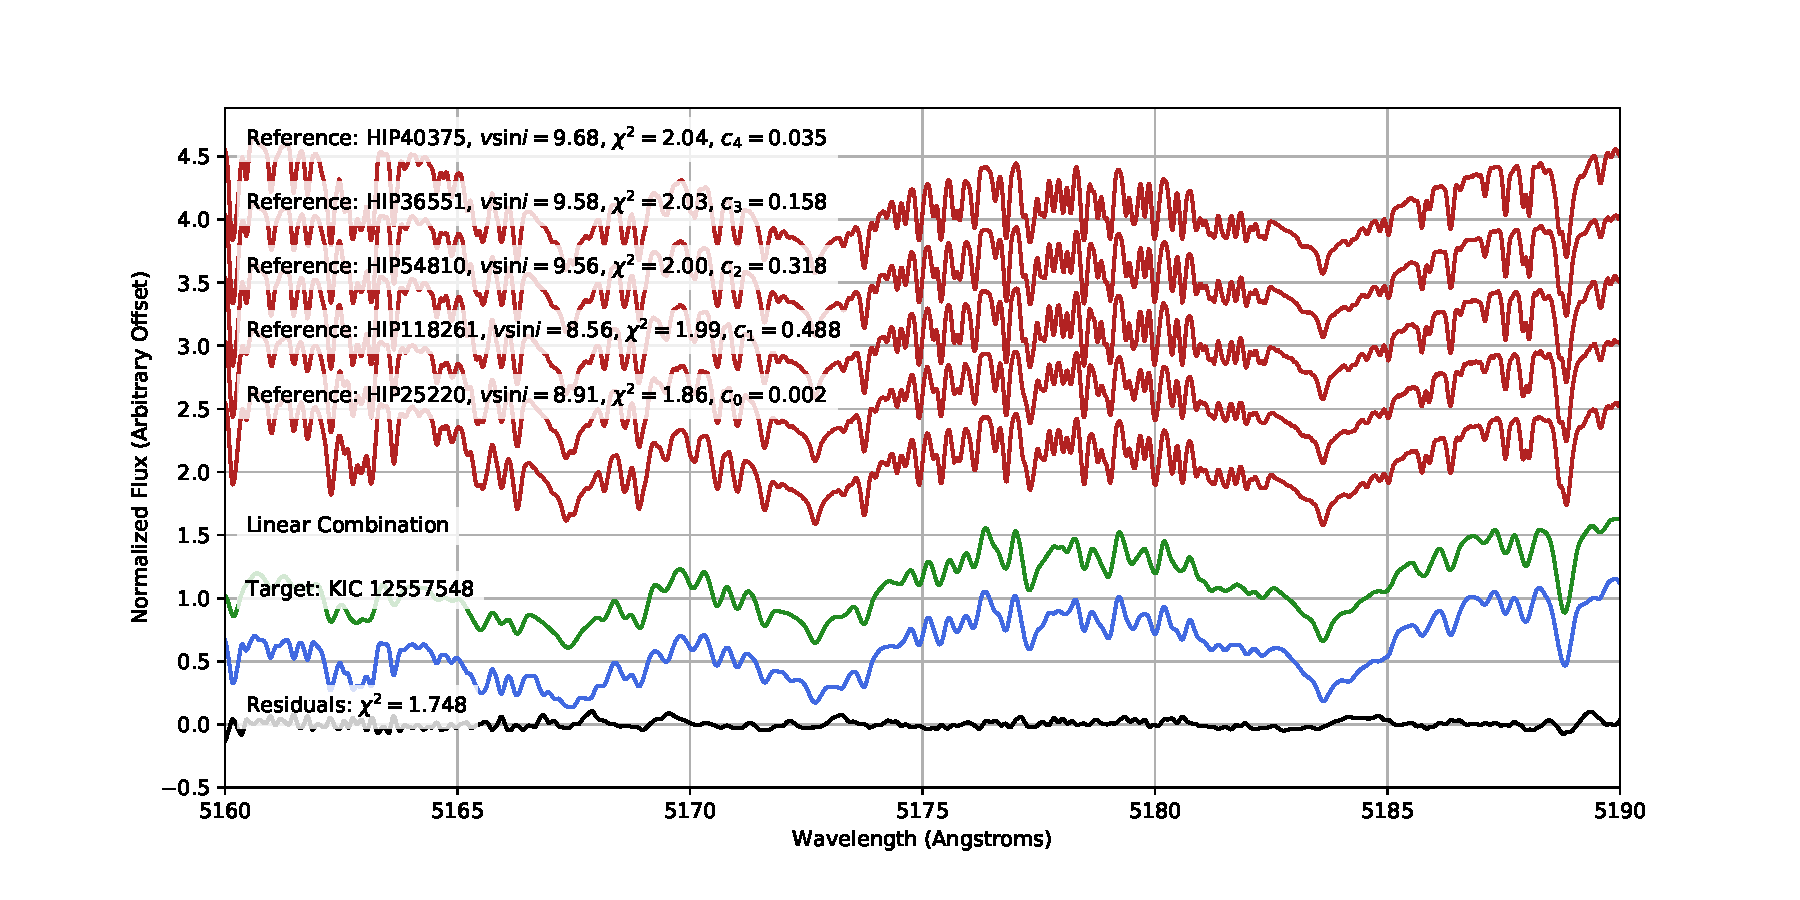
\includegraphics[width=0.8\textwidth]{images/subaru/lincomb_kic1255.pdf}
\caption{Linear combination of templates that best matches KIC 1255.}\label{fig:SpecMatch-EmpComb}
\end{centering}
\end{figure*}

We posit that the initial analysis of the 2013 Subaru spectrum \citep{kawahara2013starspots} that found a temperature and log(g) of 4950 K and 3.9 log(cm/s$^{-2}$) was affected by insufficient signal to noise in the spectrum.
The 2013 data has a 30\% smaller count rate (in e$^-$/s) than the 2015 data likely because the 2013 weather and guiding were sub-optimal.
On top of that, the total exposure time for the 2013 observations was only 1.5 hours.
The consequence of the increased noise in the 2013 spectra affected the interpretation of this high resolution spectrum.
For example, the SNR of the Na D lines was $\sim$ 30, which is near the threshold needed for the \citet{takeda2005specFGKdwarfs} equivalent width method employed in the initial analysis.
We therefore conclude that the noise in the spectrum affected the stellar parameters rather than gas absorption from sublimating dust grains.

\clearpage

\section{Kepler Re-analysis}
We examine the 17 total quarters of Kepler data for three purposes:
\begin{enumerate}
	\item To understand the statistics of the transits and put the 2013-2016 observations in context. Mainly, how likely/unlikely were the weak transits observed in 2013-2014?
	\item To measure the radius of the planet or put an upper limit on its radius by examining any possible transit beneath the dust signal
	\item Identify any new patterns or observations from the Kepler data that might occur along the way
\end{enumerate}

We downloaded all 17 quarters of Kepler Long-Cadence data from the MAST archive beginning on 2009-05-13 and ending on 2013-04-08 for a total of 1425 days or 2181.5 orbits.
The Kepler data were examined for one transit or secondary eclipse at a time with a window of $\pm$0.28 in orbital phase.
A quadratic baseline is fit to all the points before a phase of 0.12 and after a phase of 0.15 within the $\pm$ 0.28 phase window.
All points are divided by this baseline to produce a normalized flux transit or eclipse profile.
The secondary eclipses are used to quantify the noise in the transit depths.

\subsection{Kepler Secondary Eclipse}

We confirm the result of \citet{vanWerkhoven2014} that no secondary eclipse is detected a at $\lesssim 50$ ppm, seen in Figure \ref{fig:secEclipse}. 
We then use the secondary eclipses as a way to characterize the noise of the primary eclipses.
Both have the same quadratic baseline removal process over the same time intervals.

\begin{figure*}[!hbtp]
\begin{centering}
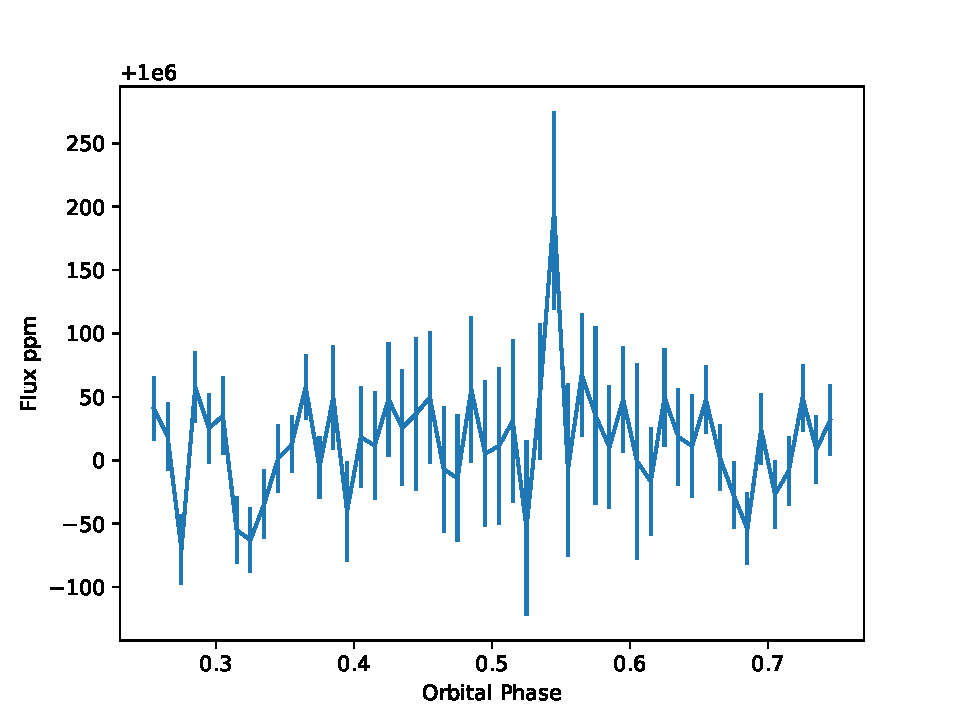
\includegraphics[width=0.45\textwidth]{images/kepler/secondary_eclipse.pdf}
\caption{No secondary eclipse ( $\lesssim$ 50 ppm) is detected from a phase range of -0.25 to 0.75, even with 17 quarters (4 years) of Kepler Long Cadence data.
Here, the data are binned to orbital phases of 0.1 (1.5 minutes) and errors calculated from the standard error in the mean of the data within a bin.
}\label{fig:secEclipse}
\end{centering}
\end{figure*}

\subsection{Average Light Curve Analysis}

In order to perform some analysis techniques on the data and to study the transit depth behavior, we first create a uniform cleaned two dimensional array of the time series.
We interpolated the Kepler long-cadence data set onto a fixed phase grid with a spacing of 15 minutes (to Nyquist sample the 30 minute observation cadence) and put together all the time series that have no gaps into this two dimensional grid.
This cleaned Kepler long-cadence array is shown in Figure \ref{fig:riverPlots}.

We start by taking the average transit light curve of all the long cadence data (the mean of the 2D grid along the transit number axis).
We then take the dot product ($\bullet$) with this average light curve to create an amplitude time series.
\begin{equation}
A = \frac{(f - 1) \bullet a}{a \bullet a},
\end{equation}
where $A$ is the amplitude vector, $f$ is the flux matrix with x indices of time and y indices of transit number and $a$ is the average spectrum.
This dot product is then multiplied by the average transit light curve to create a 2D model grid.
The residual of this model shows substantial deviations from white noise, so we explore more sophisticated models than the average light curve below.

\begin{figure*}[!hbtp]
\begin{centering}
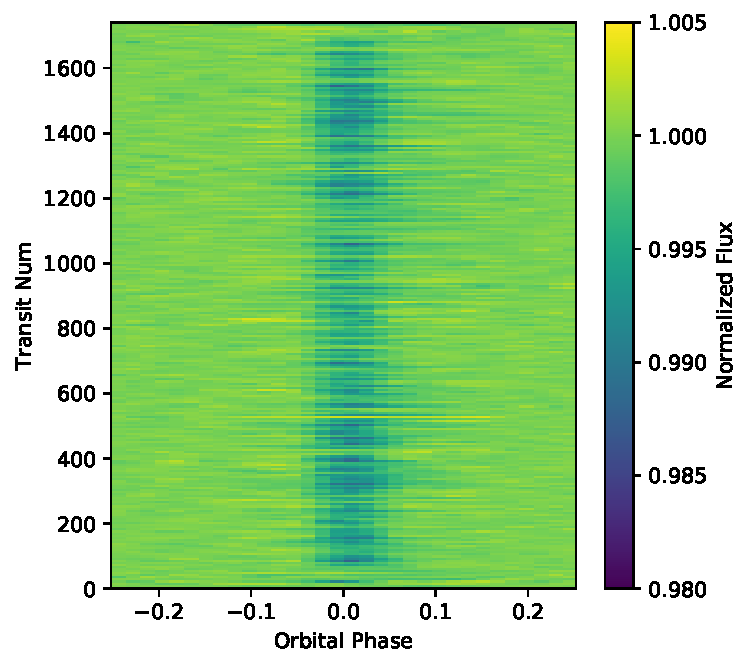
\includegraphics[width=0.32\textwidth]{images/kepler/photometry_riverplot.pdf}
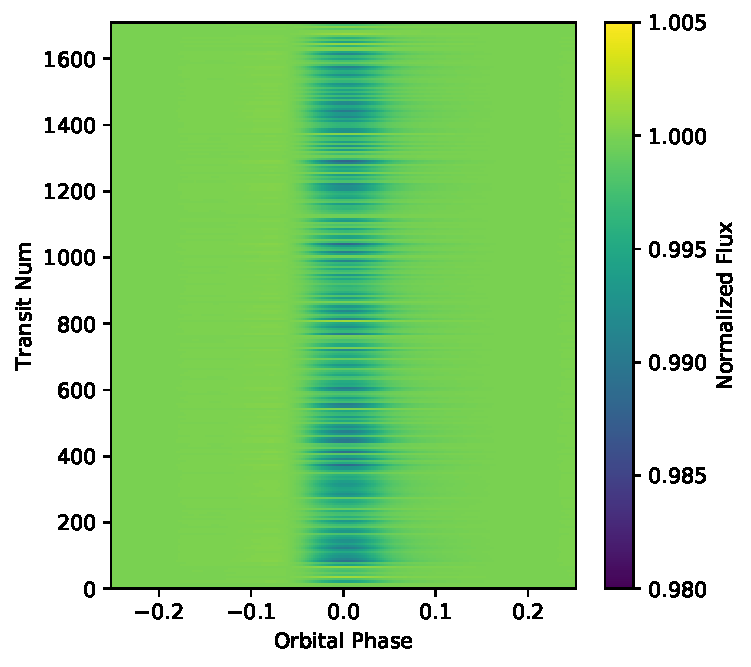
\includegraphics[width=0.32\textwidth]{images/kepler/model_riverplot.pdf}
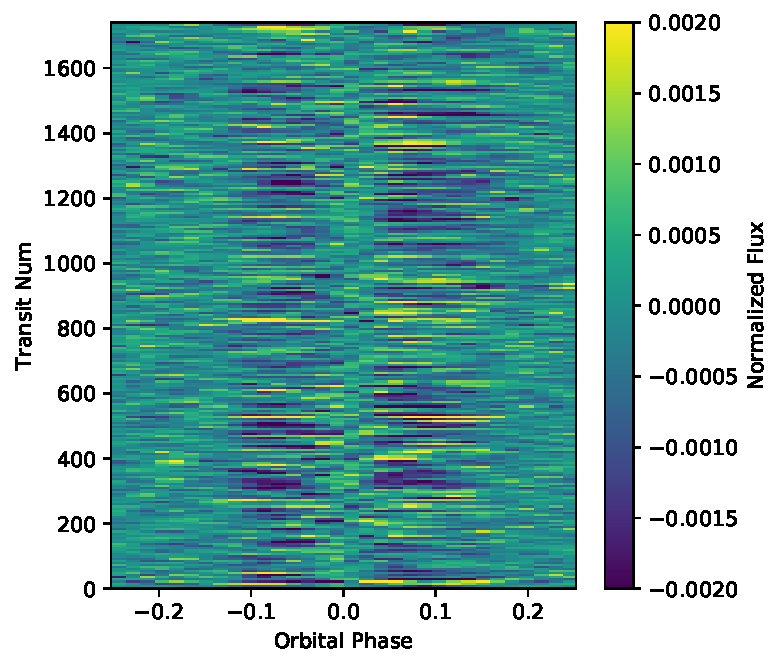
\includegraphics[width=0.32\textwidth]{images/kepler/residual_riverplot.pdf}
\caption{Cleaned Kepler Long-cadence data (Left) and model fit using the average light curve (Middle).
(Right) The residuals show significant deviations near phases of -0.5 and 0.05.
}\label{fig:riverPlots}
\end{centering}
\end{figure*}

\subsection{Principal Component Analysis}

As another way of analyzing the light curve data, we apply Principal Component Analysis (PCA) to this two dimensional grid.
Here, we are assuming that the grid of orbital phases (spaced by 15 minutes) contains random correlated variables with different realizations along the transit number axis.
The first principal component eigenvector is the linear combination of these random variables that maximizes the variance in the data.
The second principal component eigenvector is the linear combination of these random variables with the next-highest variance while being orthogonal to the first principal component.
This continues up to some finite number of principal components, with the hope that we can use just a few orthogonal light curves to adequately describe the data \citep[e.g.][]{jolliffe2002pca}.
We use the Python package \texttt{scikit-learn} \citep{pedregosa2011scikit-learn} to calculate the principal components and eigenvectors.

We use a covariance matrix as opposed to correlation matrix to calculate the principal component eigenvectors.
In other uses of PCA, the variables are often scaled so that they all have a variance of 1.0 to ensure that variables with intrinsically larger variance (such as height in inches over weight in kilograms) do not get higher loadings in the principal component vectors \citep{jolliffe2002pca}.
However, we do not scale the variables (columns) by variance and use a covariance matrix because all of our variables are the same units, flux.
If we scaled each column in this 2D grid by its standard deviation or used a correlation matrix, this would magnify the contribution of photon noise to out-of-transit data over the real astrophysical variability of the inner phases (between $\sim$-0.12 to $\sim$0.15).
\begin{figure*}[!hbtp]
\begin{centering}
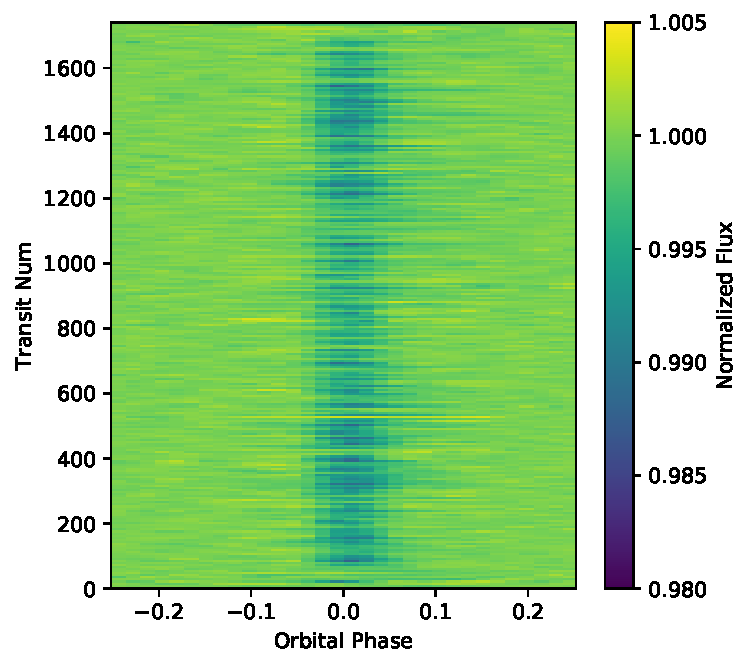
\includegraphics[width=0.32\textwidth]{images/kepler/photometry_riverplot.pdf}
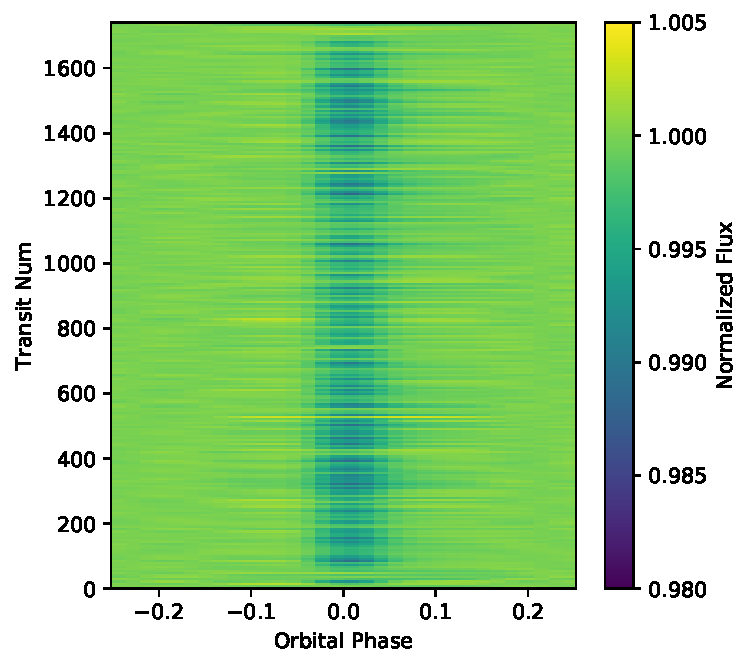
\includegraphics[width=0.32\textwidth]{images/kepler/pca_model_2D.pdf}
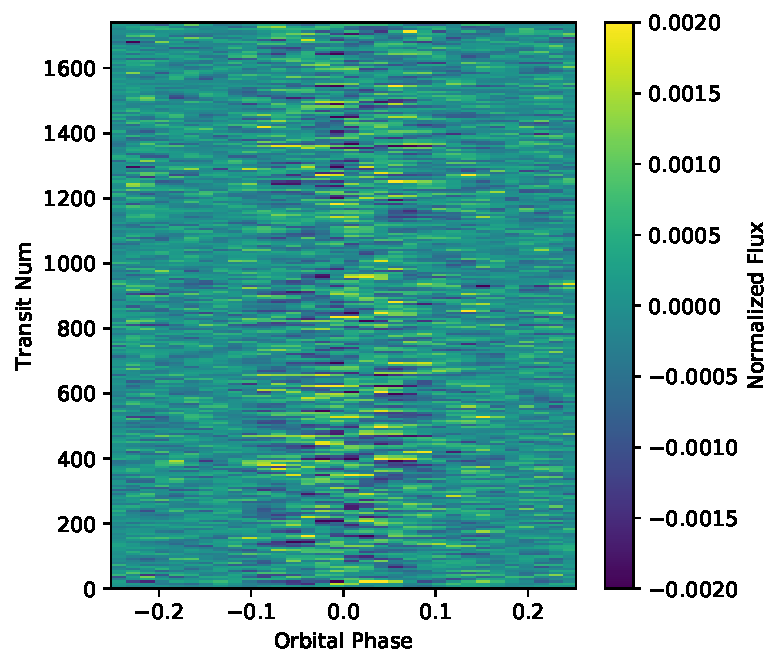
\includegraphics[width=0.32\textwidth]{images/kepler/pca_resid_2D.pdf}
\caption{Cleaned Kepler Long-cadence data (Top Left) and model fit using 4 Principal Components (Top Right).
(Right) The residuals show smaller residuals than the average model.
}\label{fig:riverPlotsPCA}
\end{centering}
\end{figure*}

Figure \ref{fig:pcaVectorsComp} shows the calculated 4 eigenvectors as a function of orbital phase and the corresponding 4 principal components as a function of transit number.
We weight each eigenvectors by the square root of the explained variance of each principal component, as is used in meteorology \citep{richman1986pcaRotation}.
The first 4 eigenvectors explain 62\%, 12\%, 6\% and 3\% of the variance (a total of 84\%) for the 32 points in the phase grid from -0.25 to 0.25.

\begin{figure*}[!hbtp]
\begin{centering}
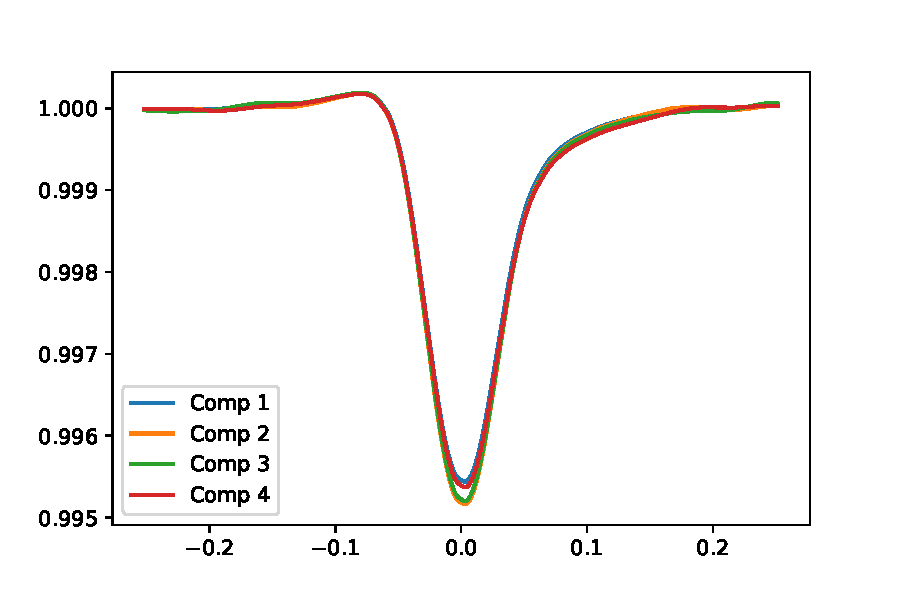
\includegraphics[width=0.49\textwidth]{images/kepler/pca_k1255.pdf}
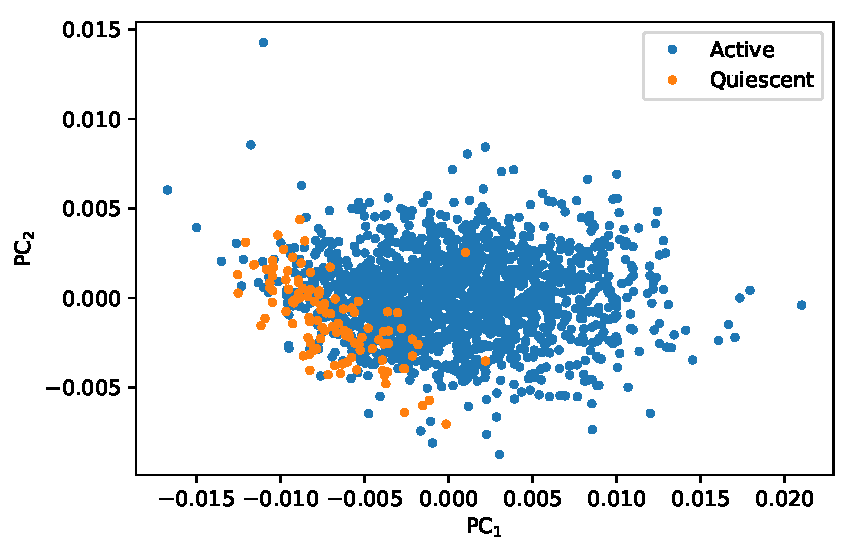
\includegraphics[width=0.49\textwidth]{images/kepler/pc1_pc2_acive_quiescent.pdf}
\caption{The principal component eigenvectors scaled by the square root of the eigenvalues (Left), shows that the first component largely describes the extinction while the second and third show the contributions from forward scattering.
The first two principal components (Right) do not isolate any separate populations of transits.
As expected, the quiescent periods show up as low principal component contributions from both of the two first two eigenvectors (ie. a flatter light curve)}\label{fig:pcaVectorsComp}
\end{centering}
\end{figure*}
Figure \ref{fig:tserPC1} shows the time series of the first principal component, which tracks well with the dot product with the average light curve.

\begin{figure*}[!hbtp]
\begin{centering}
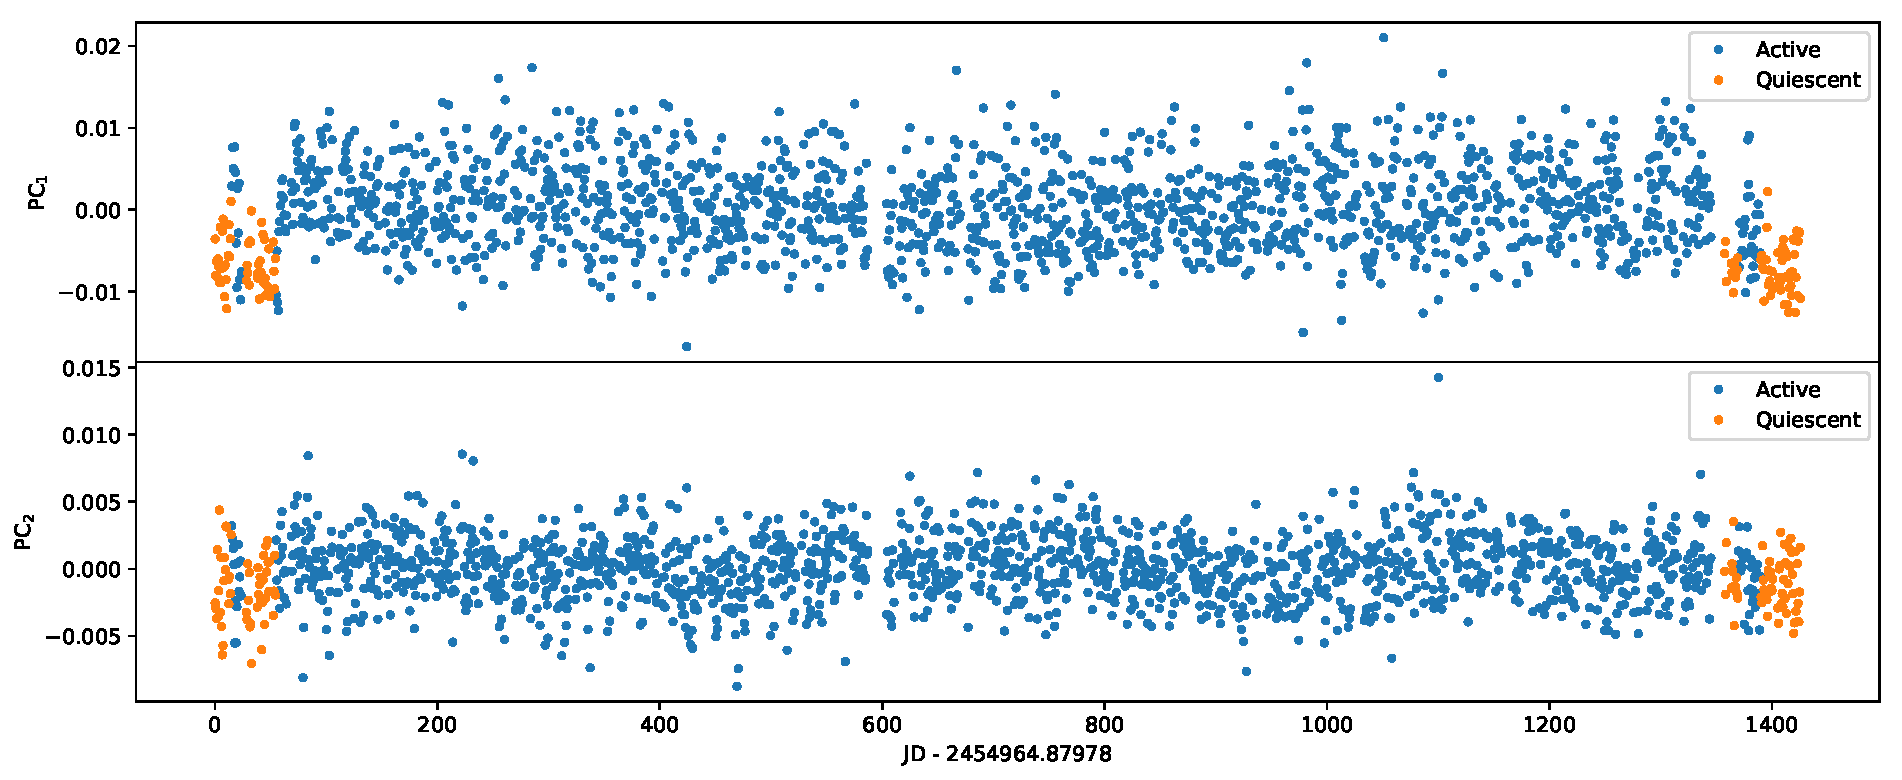
\includegraphics[width=0.99\textwidth]{images/kepler/pc_tser_w_quiescent.pdf}
\caption{The first two principal component's time series.}\label{fig:tserPC1}
\end{centering}
\end{figure*}





In Figure \ref{fig:ampPeriodogram} we show the periodogram of amplitudes that have peaks at 0.654, 22.9, 153 and 750 days.
The 22.9 day peak is consistent with the \citet{kawahara2013starspots} and \citet{croll2015starspots} that shows amplitudes are anti-correlated with stellar flux.
As suggested in \citet{kawahara2013starspots}, the anti-correlation points to a physical mechanism for the disintegration - such as magnetic activity or high energy flux associated with spots causing disintegration on the planet.

\begin{figure*}[!hbtp]
\begin{centering}
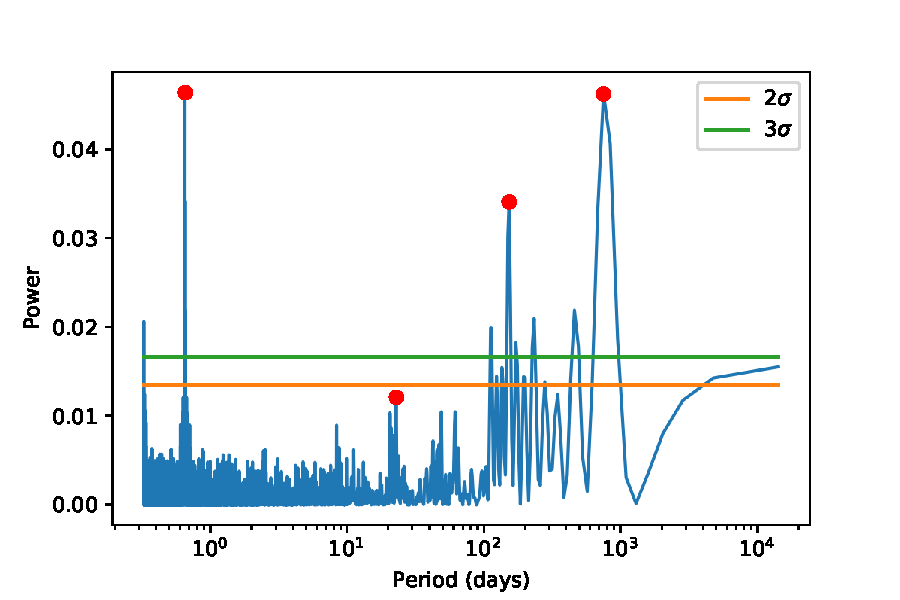
\includegraphics[width=0.49\textwidth]{images/kepler/amplitude_periodogram.pdf}
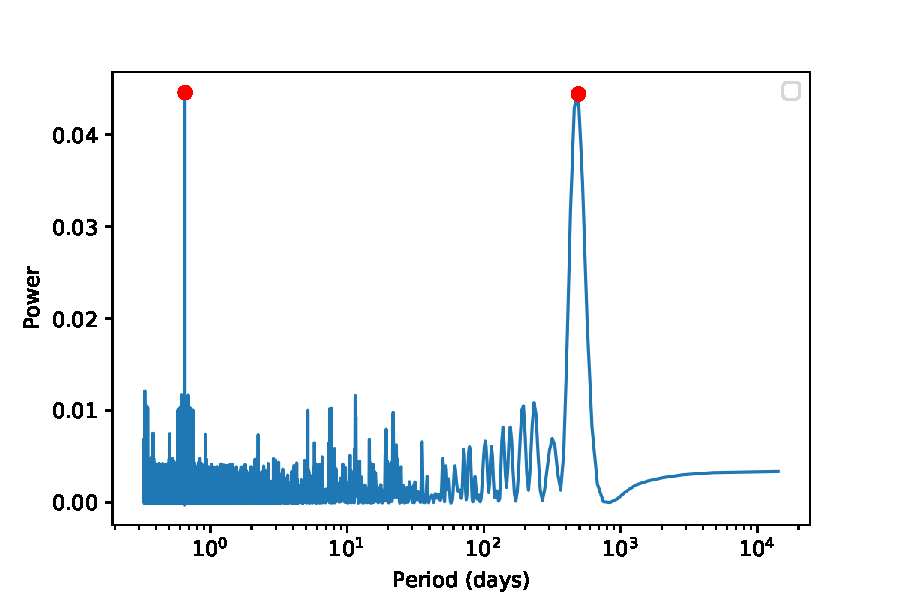
\includegraphics[width=0.49\textwidth]{images/kepler/pc2_periodogram.pdf}
\caption{Periodogram of the amplitude time series shown in Figure \ref{fig:tserPC1}
Bootstrap error estimates for the 2$\sigma$ and 3$\sigma$ confidence intervals are shown.
The peak at 0.654 days is the orbital period.
The peaks at 153 and 750 days are likely caused by the longer intervals of low disintegration activity.
The 22.9 day peak is consistent with \citet{kawahara2013starspots}, who notice that this period is co-incident with the stellar rotation period.}\label{fig:ampPeriodogram}
\end{centering}
\end{figure*}

\begin{figure*}[!hbtp]
\begin{centering}
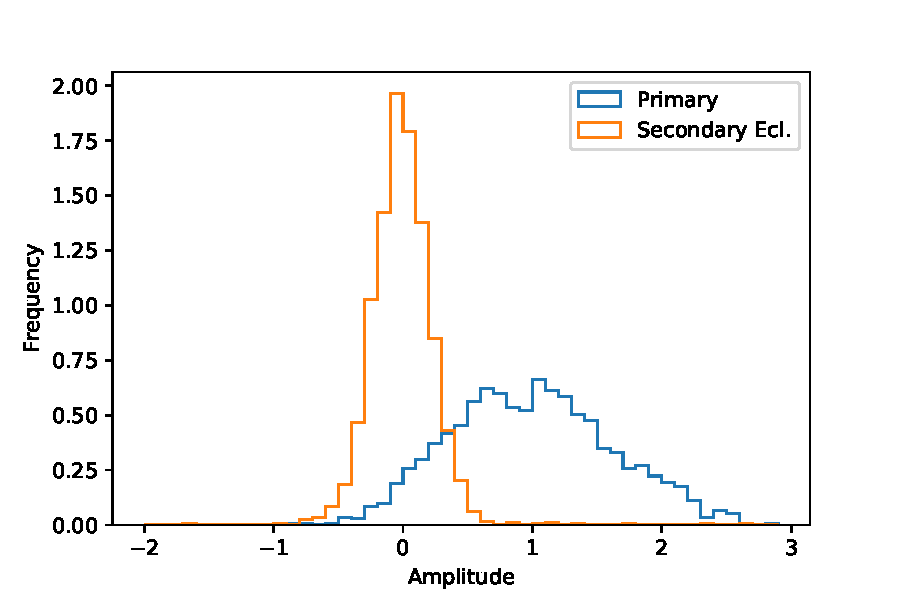
\includegraphics[width=0.49\textwidth]{images/kepler/amplitude_histogram.pdf}
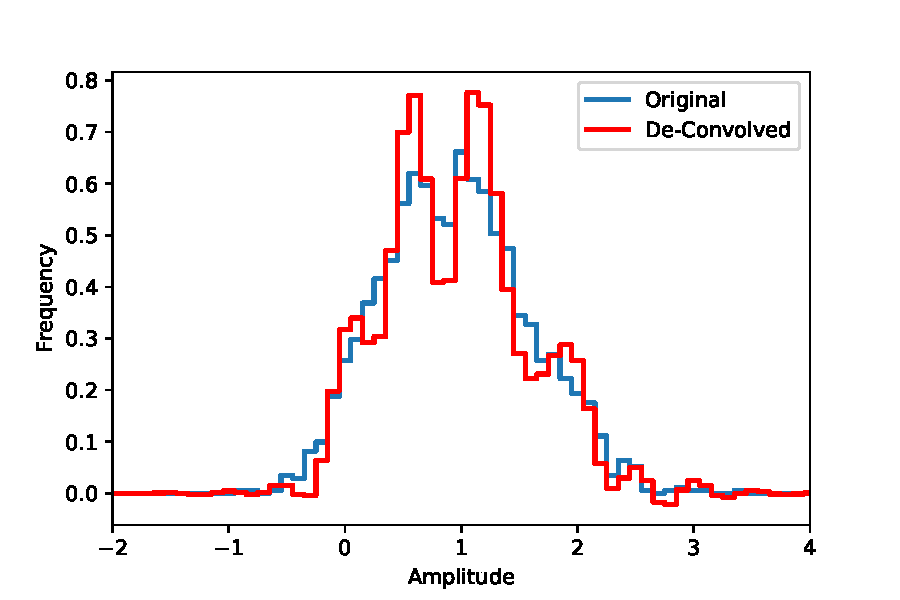
\includegraphics[width=0.49\textwidth]{images/kepler/deconvolved_hist.pdf}
\caption{(Left) Histogram of transit amplitudes.
An amplitude of 1.0 corresponds to the average light curve (with flux minimum of 99.53\% or 0.47\% transit depth).
A comparison histogram is shown from the Kepler Secondary eclipses to show the statistical noise.
(Right) The primary transit histogram is de-convolved by the secondary eclipse histogram to attempt to measure the intrinsic astrophysical variability.}\label{fig:histograms}
\end{centering}
\end{figure*}


\begin{figure*}[!hbtp]
\begin{centering}
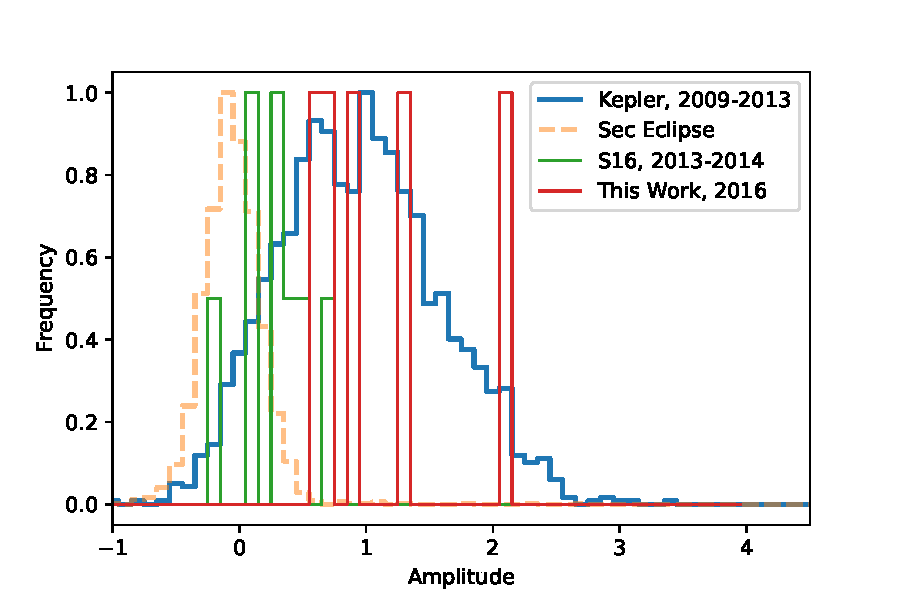
\includegraphics[width=0.49\textwidth]{images/kepler/amp_distributions_comparison.pdf}
\caption{Normalized frequency of 3 different distributions: 1) all of the Kepler Long Cadence data from 2009 to 2013, 2) the 8 night ground-based IRTF campaign in the summers of 2013 and 2014 from \citet{schlawin2016kic1255} (S16) and 3) the 5 night Kuiper observatory campaign in the summer of 2016.
The \citet{schlawin2016kic1255} (S16) events give a Kolmogorov Smirnov p value of 0.001 of the null hypothesis that the S16 results are drawn from the same distribution as the Kepler Long Cadence.
In contrast, the 2016 photometric results in this work are consistent with the Kepler Long Cadence data, giving a  p value of 0.5 of the null hypothesis.}\label{fig:histoPhot}
\end{centering}
\end{figure*}


%\begin{figure*}[!hbtp]
%\begin{centering}
%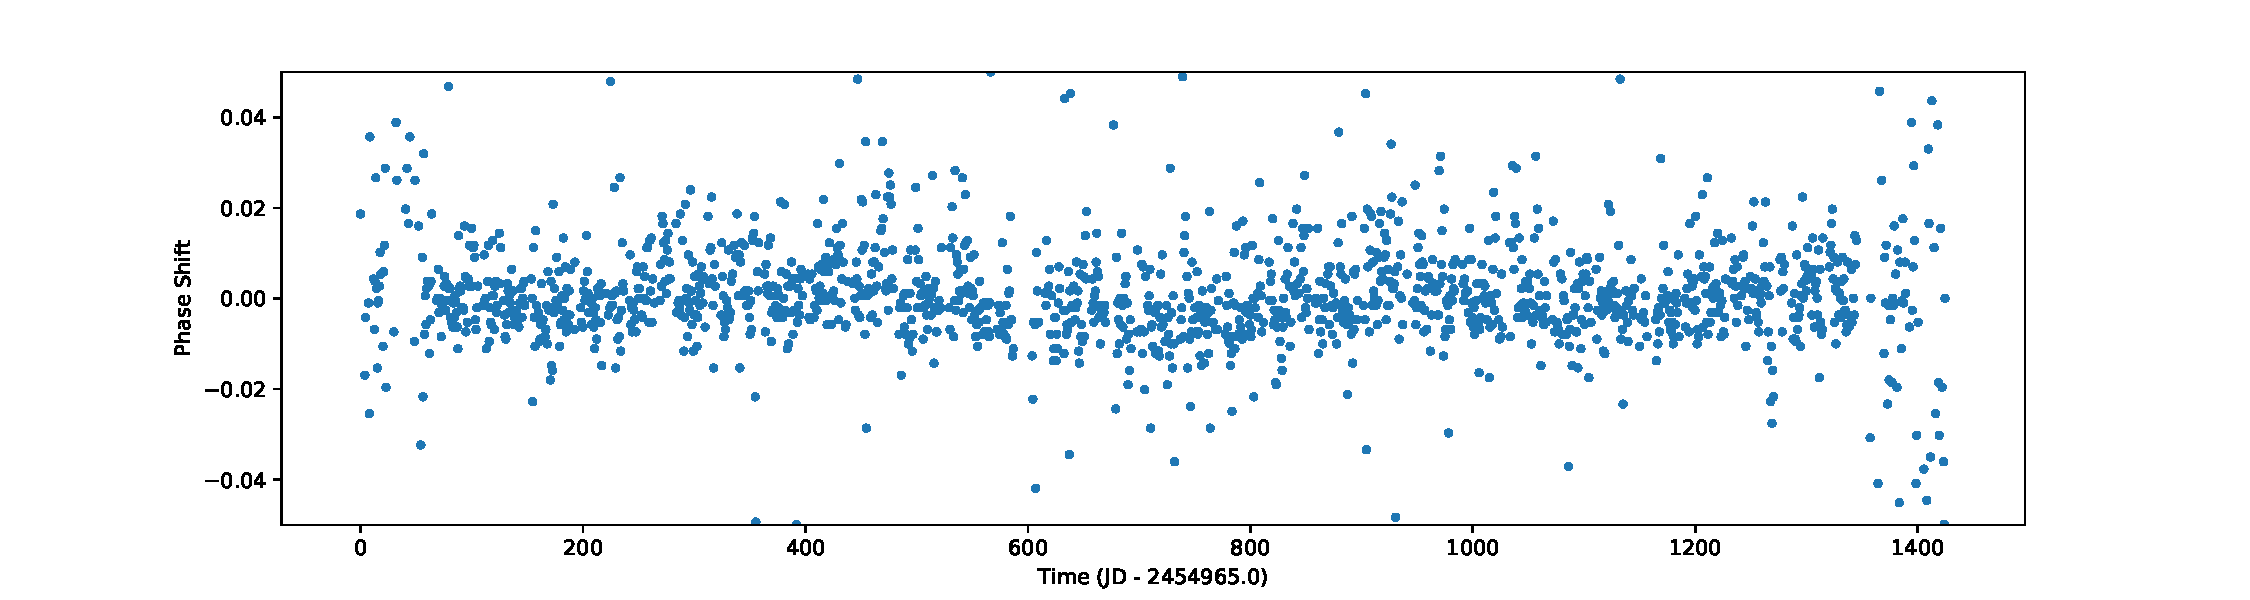
\includegraphics[width=0.99\textwidth]{images/kepler/phase_shifts.pdf}
%\caption{Time Series of phase shifts.}\label{fig:phaseShift}
%\end{centering}
%\end{figure*}
%
%
%\begin{figure*}[!hbtp]
%\begin{centering}
%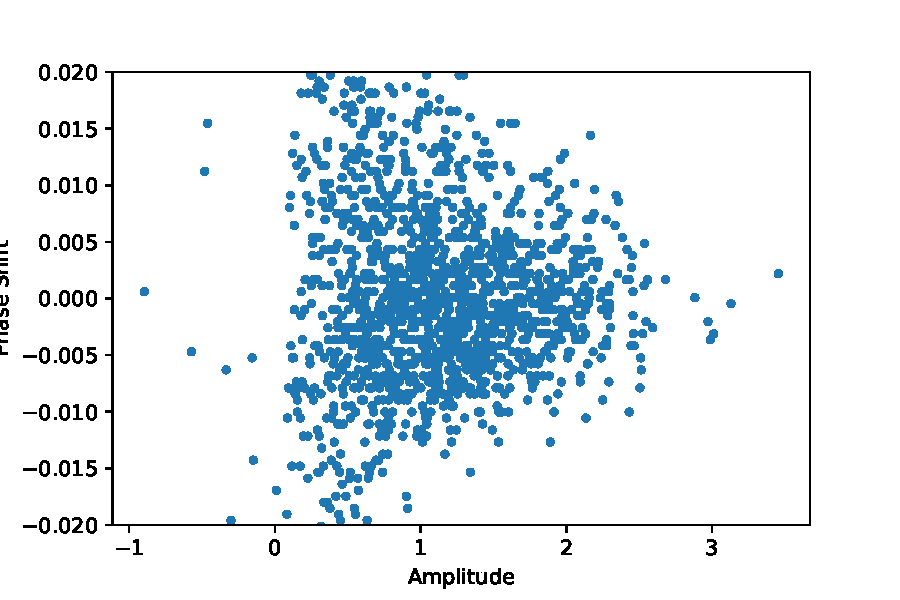
\includegraphics[width=0.49\textwidth]{images/kepler/phase_shift_vs_amplitude.pdf}
%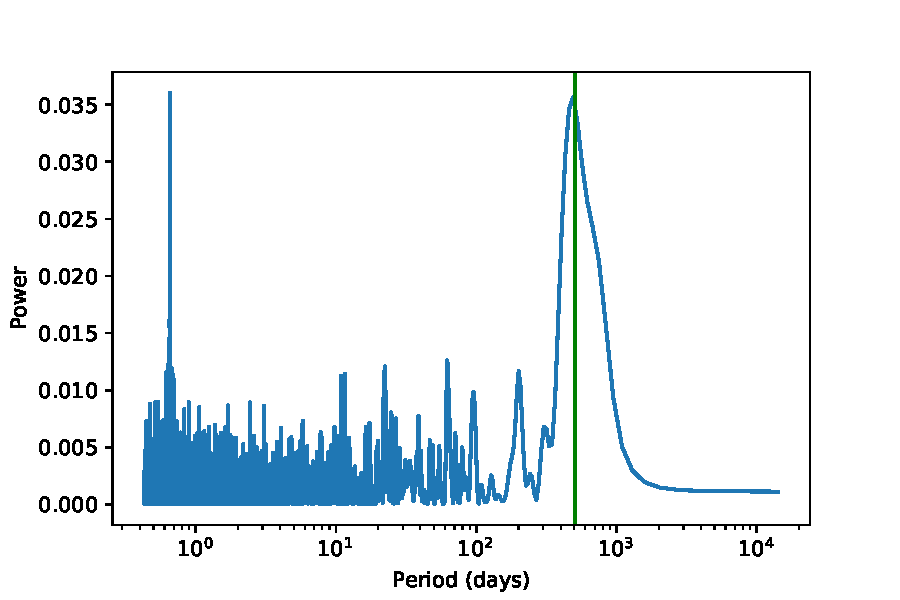
\includegraphics[width=0.49\textwidth]{images/kepler/phase_shifts_periodogram.pdf}
%\caption{Phase shifts versus amplitude (left) and phase shift periodogram (right).}\label{fig:phaseShift}
%\end{centering}
%\end{figure*}



\section{Conclusions}\label{sec:conclusions}

\section{Acknowledgements}
%Thanks to Alessondra Springman for good resources on core and mantle compositions and the gases that could sublimate off of them.
%Thanks to Jonathan Fraine and Rafia Bushra for help with observing at the 61-inch Kuiper telescope on Mt Bigelow.
%MCMC fitting makes use of \texttt{emcee} \citep{foreman-mackey2013emcee} and the covariance plot was made with \texttt{corner.py} \citep{foremanCorner}.
Thanks to Kento Masuda for sharing the 2015 Subaru spectrum of \shStar\ and giving helpful comments on this work.
Funding for the E Schlawin is provided by NASA Goddard Spaceflight Center.

%If  used, this work made use of the \texttt{astropy} package \citep{astropy2013}.
%If used, some data was collected from the Open Exoplanet Catalogue \citep{rein2012openExoCat}.

%% In a manner similar to \objectname authors can provide links to dataset
%% hosted at participating data centers via the \dataset{} command.  The
%% second curly bracket argument is printed in the text while the first
%% parentheses argument serves as the valid data set identifier.  Large
%% lists of data set are best provided in a table (see Table 3 for an example).
%% Valid data set identifiers should be obtained from the data center that
%% is currently hosting the data.
%%
%% Note that AASTeX interprets everything between the curly braces in the 
%% macro as regular text, so any special characters, e.g. "#" or "_," must be 
%% preceded by a backslash. Otherwise, you will get a LaTeX error when you 
%% compile your manuscript.  Special characters do not 
%% need to be escaped in the optional, square-bracket argument.



%% In this section, we use  the \subsection command to set off
%% a subsection.  \footnote is used to insert a footnote to the text.

%% Observe the use of the LaTeX \label
%% command after the \subsection to give a symbolic KEY to the
%% subsection for cross-referencing in a \ref command.
%% You can use LaTeX's \ref and \label commands to keep track of
%% cross-references to sections, equations, tables, and figures.
%% That way, if you change the order of any elements, LaTeX will
%% automatically renumber them.

%% This section also includes several of the displayed math environments
%% mentioned in the Author Guide.


%% The equation environment wil produce a numbered display equation.


%% The \notetoeditor{TEXT} command allows the author to communicate
%% information to the copy editor.  This information will appear as a
%% footnote on the printed copy for the manuscript style file.  Nothing will
%% appear on the printed copy if the preprint or
%% preprint2 style files are used.

%% The eqnarray environment produces multi-line display math. The end of
%% each line is marked with a \\. Lines will be numbered unless the \\
%% is preceded by a \nonumber command.
%% Alignment points are marked by ampersands (&). There should be two
%% ampersands (&) per line.

%% Putting eqnarrays or equations inside the mathletters environment groups
%% the enclosed equations by letter. For instance, the eqnarray below, instead
%% of being numbered, say, (4) and (5), would be numbered (4a) and (4b).
%% LaTeX the paper and look at the output to see the results.

%% This section contains more display math examples, including unnumbered
%% equations (displaymath environment). The last paragraph includes some
%% examples of in-line math featuring a couple of the AASTeX symbol macros.

%% The displaymath environment will produce the same sort of equation as
%% the equation environment, except that the equation will not be numbered
%% by LaTeX.
%% If you wish to include an acknowledgments section in your paper,
%% separate it off from the body of the text using the \acknowledgments
%% command.

%% Included in this acknowledgments section are examples of the
%% AASTeX hypertext markup commands. Use \url without the optional [HREF]
%% argument when you want to print the url directly in the text. Otherwise,
%% use either \url or \anchor, with the HREF as the first argument and the
%% text to be printed in the second.

\acknowledgments



%% To help institutions obtain information on the effectiveness of their
%% telescopes, the AAS Journals has created a group of keywords for telescope
%% facilities. A common set of keywords will make these types of searches
%% significantly easier and more accurate. In addition, they will also be
%% useful in linking papers together which utilize the same telescopes
%% within the framework of the National Virtual Observatory.
%% See the AASTeX Web site at http://aastex.aas.org/
%% for information on obtaining the facility keywords.

%% After the acknowledgments section, use the following syntax and the
%% \facility{} macro to list the keywords of facilities used in the research
%% for the paper.  Each keyword will be checked against the master list during
%% copy editing.  Individual instruments or configurations can be provided 
%% in parentheses, after the keyword, but they will not be verified.

%{\it Facilities:} \facility{Nickel}, \facility{HST (STIS)}, \facility{CXO (ASIS)}.

\facility{Subaru}

\software{
	\texttt{ccdproc} \citep{craig2015ccdproc},
	\texttt{astropy} \citep{astropy2013}, 
	\texttt{scikit-learn} \citep{pedregosa2011scikit-learn},
	\texttt{photutils v0.3} \citep{bradley2016photutilsv0p3},
	\texttt{iraf},
	\texttt{SpecMatch-Emp} \citep{yee2017specMatch} 
          %\texttt{emcee} \citep{foreman-mackey2013emcee}, 
          }


%% Appendix material should be preceded with a single \appendix command.
%% There should be a \section command for each appendix. Mark appendix
%% subsections with the same markup you use in the main body of the paper.

%% Each Appendix (indicated with \section) will be lettered A, B, C, etc.
%% The equation counter will reset when it encounters the \appendix
%% command and will number appendix equations (A1), (A2), etc.

\appendix

%% The reference list follows the main body and any appendices.
%% Use LaTeX's thebibliography environment to mark up your reference list.
%% Note \begin{thebibliography} is followed by an empty set of
%% curly braces.  If you forget this, LaTeX will generate the error
%% "Perhaps a missing \item?".
%%
%% thebibliography produces citations in the text using \bibitem-\cite
%% cross-referencing. Each reference is preceded by a
%% \bibitem command that defines in curly braces the KEY that corresponds
%% to the KEY in the \cite commands (see the first section above).
%% Make sure that you provide a unique KEY for every \bibitem or else the
%% paper will not LaTeX. The square brackets should contain
%% the citation text that LaTeX will insert in
%% place of the \cite commands.

%% We have used macros to produce journal name abbreviations.
%% AASTeX provides a number of these for the more frequently-cited journals.
%% See the Author Guide for a list of them.

%% Note that the style of the \bibitem labels (in []) is slightly
%% different from previous examples.  The natbib system solves a host
%% of citation expression problems, but it is necessary to clearly
%% delimit the year from the author name used in the citation.
%% See the natbib documentation for more details and options.

\bibliographystyle{apj}
\bibliography{ms}

%\clearpage

%% Use the figure environment and \plotone or \plottwo to include
%% figures and captions in your electronic submission.
%% To embed the sample graphics in
%% the file, uncomment the \plotone, \plottwo, and
%% \includegraphics commands
%%
%% If you need a layout that cannot be achieved with \plotone or
%% \plottwo, you can invoke the graphicx package directly with the
%% \includegraphics command or use \plotfiddle. For more information,
%% please see the tutorial on "Using Electronic Art with AASTeX" in the
%% documentation section at the AASTeX Web site, http://aastex.aas.org/
%%
%% The examples below also include sample markup for submission of
%% supplemental electronic materials. As always, be sure to check
%% the instructions to authors for the journal you are submitting to
%% for specific submissions guidelines as they vary from
%% journal to journal.

%% This example uses \plotone to include an EPS file scaled to
%% 80% of its natural size with \epsscale. Its caption
%% has been written to indicate that additional figure parts will be
%% available in the electronic journal.

%\begin{figure}
%\epsscale{.80}
%\plotone{f1.eps}
%\caption{Derived spectra for 3C138 \citep[see][]{heiles03}. Plots for all sources are available
%in the electronic edition of {\it The Astrophysical Journal}.\label{fig1}}
%\end{figure}

%\clearpage

%% Here we use \plottwo to present two versions of the same figure,
%% one in black and white for print the other in RGB color
%% for online presentation. Note that the caption indicates
%% that a color version of the figure will be available online.
%%

%\begin{figure}
%\plottwo{f2.eps}{f2_color.eps}
%\caption{A panel taken from Figure 2 of \citet{rudnick03}. 
%See the electronic edition of the Journal for a color version 
%of this figure.\label{fig2}}
%\end{figure}

%% This figure uses \includegraphics to scale and rotate the still frame
%% for an mpeg animation.

%\begin{figure}
%\includegraphics[angle=90,scale=.50]{f3.eps}
%\caption{Animation still frame taken from \citet{kim03}.
%This figure is also available as an mpeg
%animation in the electronic edition of the
%{\it Astrophysical Journal}.}
%\end{figure}

%% If you are not including electonic art with your submission, you may
%% mark up your captions using the \figcaption command. See the
%% User Guide for details.
%%
%% No more than seven \figcaption commands are allowed per page,
%% so if you have more than seven captions, insert a \clearpage
%% after every seventh one.

%% Tables should be submitted one per page, so put a \clearpage before
%% each one.

%% Two options are available to the author for producing tables:  the
%% deluxetable environment provided by the AASTeX package or the LaTeX
%% table environment.  Use of deluxetable is preferred.
%%

%% Three table samples follow, two marked up in the deluxetable environment,
%% one marked up as a LaTeX table.

%% In this first example, note that the \tabletypesize{}
%% command has been used to reduce the font size of the table.
%% We also use the \rotate command to rotate the table to
%% landscape orientation since it is very wide even at the
%% reduced font size.
%%
%% Note also that the \label command needs to be placed
%% inside the \tablecaption.

%% This table also includes a table comment indicating that the full
%% version will be available in machine-readable format in the electronic
%% edition.

%% If you use the table environment, please indicate horizontal rules using
%% \tableline, not \hline.
%% Do not put multiple tabular environments within a single table.
%% The optional \label should appear inside the \caption command.



%% If the table is more than one page long, the width of the table can vary
%% from page to page when the default \tablewidth is used, as below.  The
%% individual table widths for each page will be written to the log file; a
%% maximum tablewidth for the table can be computed from these values.
%% The \tablewidth argument can then be reset and the file reprocessed, so
%% that the table is of uniform width throughout. Try getting the widths
%% from the log file and changing the \tablewidth parameter to see how
%% adjusting this value affects table formatting.

%% The \dataset{} macro has also been applied to a few of the objects to
%% show how many observations can be tagged in a table.


%% Tables may also be prepared as separate files. See the accompanying
%% sample file table.tex for an example of an external table file.
%% To include an external file in your main document, use the \input
%% command. Uncomment the line below to include table.tex in this
%% sample file. (Note that you will need to comment out the \documentclass,
%% \begin{document}, and \end{document} commands from table.tex if you want
%% to include it in this document.)

%% \input{table}

%% The following command ends your manuscript. LaTeX will ignore any text
%% that appears after it.

\end{document}

%%
%% End of file `sample.tex'.
